%% Преамбула TeX-файла

% 1. Стиль и язык
\documentclass[utf8x, 14pt]{G7-32} % Стиль (по умолчанию будет 14pt)


% Остальные стандартные настройки убраны в preamble.inc.tex.
\sloppy

% Настройки стиля ГОСТ 7-32
% Для начала определяем, хотим мы или нет, чтобы рисунки и таблицы нумеровались в пределах раздела, или нам нужна сквозная нумерация.
\EqInChapter % формулы будут нумероваться в пределах раздела
\TableInChapter % таблицы будут нумероваться в пределах раздела
\PicInChapter % рисунки будут нумероваться в пределах раздела

% Добавляем гипертекстовое оглавление в PDF
\usepackage[
bookmarks=true, colorlinks=true, unicode=true,
urlcolor=black,linkcolor=black, anchorcolor=black,
citecolor=black, menucolor=black, filecolor=black,
]{hyperref}

\usepackage{listings}

\AfterHyperrefFix

\usepackage{microtype}% полезный пакет для микротипографии, увы под xelatex мало чего умеет, но под pdflatex хорошо улучшает читаемость

% Тире могут быть невидимы в Adobe Reader
\ifInvisibleDashes
\MakeDashesBold
\fi

\usepackage{graphicx}   % Пакет для включения рисунков

% С такими оно полями оно работает по-умолчанию:
% \RequirePackage[left=20mm,right=10mm,top=20mm,bottom=20mm,headsep=0pt,includefoot]{geometry}
% Если вас тошнит от поля в 10мм --- увеличивайте до 20-ти, ну и про переплёт не забывайте:
\geometry{right=10mm}
\geometry{left=30mm}
\geometry{bottom=20mm}
\geometry{ignorefoot}% считать от нижней границы текста


% Пакет Tikz
\usepackage{tikz}
\usetikzlibrary{arrows,positioning,shadows}

% Произвольная нумерация списков.
\usepackage{enumerate}

% ячейки в несколько строчек
\usepackage{multirow}

% itemize внутри tabular
\usepackage{paralist,array}

%\setlength{\parskip}{1ex plus0.5ex minus0.5ex} % разрыв между абзацами
\setlength{\parskip}{1ex} % разрыв между абзацами
\usepackage{blindtext}

% Центрирование подписей к плавающим окружениям
%\usepackage[justification=centering]{caption}

\usepackage{newfloat}
\DeclareFloatingEnvironment[
placement={!ht},
name=Equation
]{eqndescNoIndent}
\edef\fixEqndesc{\noexpand\setlength{\noexpand\parindent}{\the\parindent}\noexpand\setlength{\noexpand\parskip}{\the\parskip}}
\newenvironment{eqndesc}[1][!ht]{%
    \begin{eqndescNoIndent}[#1]%
\fixEqndesc%
}
{\end{eqndescNoIndent}}




% Настройки листингов.
\ifPDFTeX
% 8 Листинги

\usepackage{listings}

% Значения по умолчанию
\lstset{
  basicstyle= \footnotesize,
  breakatwhitespace=true,% разрыв строк только на whitespacce
  breaklines=true,       % переносить длинные строки
%   captionpos=b,          % подписи снизу -- вроде не надо
  inputencoding=koi8-r,
  numbers=left,          % нумерация слева
  xleftmargin=17pt,
  numberstyle=\footnotesize,
  showspaces=false,      % показывать пробелы подчеркиваниями -- идиотизм 70-х годов
  showstringspaces=false,
  showtabs=false,        % и табы тоже
  stepnumber=1,
  tabsize=4,              % кому нужны табы по 8 символов?
  frame=single
}

% Стиль для псевдокода: строчки обычно короткие, поэтому размер шрифта побольше
\lstdefinestyle{pseudocode}{
  basicstyle=\small,
  keywordstyle=\color{black}\bfseries\underbar,
  language=Pseudocode,
  numberstyle=\footnotesize,
  commentstyle=\footnotesize\it
}

% Стиль для обычного кода: маленький шрифт
\lstdefinestyle{realcode}{
  basicstyle=\scriptsize,
  numberstyle=\footnotesize
}

% Стиль для коротких кусков обычного кода: средний шрифт
\lstdefinestyle{simplecode}{
  basicstyle=\footnotesize,
  numberstyle=\footnotesize
}

% Стиль для BNF
\lstdefinestyle{grammar}{
  basicstyle=\footnotesize,
  numberstyle=\footnotesize,
  stringstyle=\bfseries\ttfamily,
  language=BNF
}

% Определим свой язык для написания псевдокодов на основе Python
\lstdefinelanguage[]{Pseudocode}[]{Python}{
  morekeywords={each,empty,wait,do},% ключевые слова добавлять сюда
  morecomment=[s]{\{}{\}},% комменты {а-ля Pascal} смотрятся нагляднее
  literate=% а сюда добавлять операторы, которые хотите отображать как мат. символы
    {->}{\ensuremath{$\rightarrow$}~}2%
    {<-}{\ensuremath{$\leftarrow$}~}2%
    {:=}{\ensuremath{$\leftarrow$}~}2%
    {<--}{\ensuremath{$\Longleftarrow$}~}2%
}[keywords,comments]

% Свой язык для задания грамматик в BNF
\lstdefinelanguage[]{BNF}[]{}{
  morekeywords={},
  morecomment=[s]{@}{@},
  morestring=[b]",%
  literate=%
    {->}{\ensuremath{$\rightarrow$}~}2%
    {*}{\ensuremath{$^*$}~}2%
    {+}{\ensuremath{$^+$}~}2%
    {|}{\ensuremath{$|$}~}2%
}[keywords,comments,strings]

% Подписи к листингам на русском языке.
\renewcommand\lstlistingname{Листинг}
\renewcommand\lstlistlistingname{Листинги}

\else
\usepackage{local-minted}
\fi

% Полезные макросы листингов.
% Любимые команды
\newcommand{\Code}[1]{\textbf{#1}}


% Стиль титульного листа и заголовки
\usepackage{pdfpages}

\usepackage{float}

\usepackage{algorithm2e}
\SetKwInput{KwData}{Исходные параметры}
\SetKwInput{KwResult}{Результат}
\SetKwInput{KwIn}{Входные данные}
\SetKwInput{KwOut}{Выходные данные}
\SetKwIF{If}{ElseIf}{Else}{если}{тогда}{иначе если}{иначе}{конец условия}
\SetKwFor{While}{до тех пор, пока}{выполнять}{конец цикла}
\SetKw{KwTo}{от}
\SetKw{KwRet}{возвратить}
\SetKw{Return}{возвратить}
\SetKwBlock{Begin}{начало блока}{конец блока}
\SetKwSwitch{Switch}{Case}{Other}{Проверить значение}{и выполнить}{вариант}{в противном случае}{конец варианта}{конец проверки значений}
\SetKwFor{For}{цикл}{выполнять}{конец цикла}
\SetKwFor{ForEach}{для каждого}{выполнять}{конец цикла}
\SetKwRepeat{Repeat}{повторять}{до тех пор, пока}
\SetAlgorithmName{Алгоритм}{алгоритм}{Список алгоритмов}

\begin{document}

\frontmatter % выключает нумерацию ВСЕГО; здесь начинаются ненумерованные главы: реферат, введение, глоссарий, сокращения и прочее.

%\maketitle %создает титульную страницу



%\listoffigures                         % Список рисунков

%\listoftables                          % Список таблиц

%\NormRefs % Нормативные ссылки 
% Команды \breakingbeforechapters и \nonbreakingbeforechapters
% управляют разрывом страницы перед главами.
% По-умолчанию страница разрывается.

% \nobreakingbeforechapters
% \breakingbeforechapters
%\newcommand{\HRule}{\rule{\linewidth}{0.5mm}}
\fontsize{14}{14pt}\selectfont
\begin{center}

\textsc{
Министерство науки и высшего образования Российской Федерации
Федеральное государственное бюджетное образовательное учреждение 
высшего образования\\
<<Московский государственный технический университет имени Н.\,Э.~Баумана>>\\
(национальный исследовательский университет)\\
(МГТУ им. Н.Э.Баумана)\\}


\includegraphics[scale=0.5]{tex/bmstu-logo.png}\\

\textsc{Факультет <<Информатика и системы управления>>}\\
\textsc{Кафедра <<Программное обеспечение ЭВМ и информационные технологии>>}\\[1cm]

\textsc{\large \bfseries РАСЧЕТНО-ПОЯСНИТЕЛЬНАЯ ЗАПИСКА\\К ВЫПУСКНОЙ КВАЛИФИКАЦИОННОЙ РАБОТЕ\\НА ТЕМУ:}\\[1cm]

\textsc{\large Метод генерации трехмерной модели черепа по МРТ снимкам головы человека}

\vfill

\begin{flushright}
  \begin{tabular}{rll}
    Студент ИУ7-83Б & \underline{\hspace{6cm}} & А.~А.~Наместник\\[0.5cm]
    Руководитель ВКР & \underline{\hspace{6cm}} & М.~В.~Филиппов\\[0.5cm]
    Консультант & \underline{\hspace{6cm}} & Ю.~М.~Гаврилова\\ [0.5cm]
    Нормоконтролер & \underline{\hspace{6cm}} & Ю.~В.~Строганов\\[0.5cm]
  \end{tabular}
\end{flushright}

{\large Москва, \the\year}

\end{center}

\pagenumbering{gobble}
\newpage
\pagenumbering{arabic}

\includepdf[pages={-}]{Title.pdf} 
\setcounter{page}{5}
% Также можно использовать \Referat, как в оригинале
\begin{abstract}

    Расчетно-пояснительная записка содержит \pageref{LastPage}\,страниц%
    \ifnum \totfig >0
    , \totfig~рисунков%
    \fi
    \ifnum \tottab >0
    , \tottab~таблиц%
    \fi
    %
    \ifnum \totbib >0
    , \totbib~источников%
    \fi
    %
    \ifnum \totapp >0
    , \totapp~приложений.%
    \else
    .%
    \fi

Ключевые слова: MIDI, NoSQL, MongoDB, BsonDocument, хранение.

Цель бакалаврской работы - разработка метода распределенного хранения аудио-файлов в NoSQL-базе данных.

Задачи, решаемые в работе:

\begin{enumerate}
    \item Рассмотреть способы представления звуковой информации и проанализировать существующие аудио-форматы.
    \item Проанализировать способы хранения аудио-файлов в различных базах данных.
    \item Разработать метод хранения аудио-файлов.
    \item Разработать программное обеспечение, реализующее разработанный метод.
    \item Исследовать зависимость времени работы метода от количества дорожек в аудио-файле.
\end{enumerate}

Область применения разрабатываемого метода - работа с аудио-файлами формата MIDI в музыкальной индустрии.

В данной выпускной бакалаврской работе проанализированы существующие аудио-форматы, выбран аудио-формат, дающий наиболее полную информацию о музыке, проанализированы существующие решения хранения такого формата в различных базах данных и выбран способ хранения, наиболее оптимальный для выбранного формата, проанализированы существующие модели данных и выбрана наиболее подходящая под выбранный способ хранения модель, а также выбрана база данных, которая ее использует. Разработано программное обеспечение, реализующее описанный метод. Произведено исследование времени работы метода и проанализированы полученные результаты.

%%% Local Variables: 
%%% mode: latex
%%% TeX-master: "rpz"
%%% End: 
\end{abstract} 

\tableofcontents

\printnomenclature % Автоматический список сокращений

%\chapter{Обозначения и сокращения}




\Introduction
Работа с аудио-файлами сложного содержания, включающего не только оцифрованный звук, но и наборы инструкций для воспроизведения звука, требует постоянного обращения к их внутренней структуре, что может быть экономически и, с точки зрения производительности, дорогостоящей операцией. Чтобы избежать накладных расходов, которые может повлечь многократное использование сторонних приложений для работы с аудио-файлами, важно рассмотреть хранение таких файлов в удобном формате, подходящем под устанавливаемые требования использования.

Цель этой работы - разработать и реализовать метод распределенного хранения аудио-файлов в NoSQL-базе данных.

В рамках работы требуется решить следующие задачи.
\begin{enumerate}
    \item Рассмотреть способы представления звуковой информации и проанализировать существующие аудио-форматы.
    \item Проанализировать способы хранения аудио-файлов в различных базах данных.
    \item Разработать метод хранения аудио-файлов.
    \item Разработать программное обеспечение, реализующее разработанный метод.
    \item Исследовать зависимость времени работы метода от количества дорожек в аудио-файле.
\end{enumerate}


\mainmatter % это включает нумерацию глав и секций в документе ниже

\chapter{Аналитический раздел}
\label{cha:analysis}

\section{Анализ предметной области}

\subsection{Представление звуковой информации}

Звук --- это физическое явление, представляющее собой распространение упругих волн механических колебаний в твёрдой, жидкой или газообразной среде \cite{WIS}. Звуковая волна характеризуется меняющейся амплитудой и частотой \cite{SoundVolume} и воспринимается человеком с помощью органов слуха. 
Существует два способа представления звуков: прямая передача звука, при которой звук, передаваемый через электроакустический преобразователь, например, микрофон, обрабатывается и хранится таким образом, чтобы отображать исходные механические колебания; через набор параметров, описывающих звуки, которые можно использовать для воссоздания звука.

Физическим характеристикам звуковой волны соответствуют физиологические характеристики, связанные со слуховыми ощущениями человека \cite{TS}. Например, амплитуда звуковых колебаний воспринимается человеком как громкость \cite{SoundVolume}, а частота колебаний как высота тона звука \cite{FRHH}. Здоровый молодой человек способен слышать звуковые колебания в диапазоне частот от 20 Гц до 20 кГц \cite{FRHH}, что соответствует 20 --- 20 000 колебаний в секунду, однако между людьми существуют значительные различия, особенно на высоких частотах, и постепенная потеря чувствительности к более высоким частотам с возрастом считается нормой. При записи и последующем воспроизведении звука производится ряд преобразований сигнала, характер которых изменяется в зависимости от выбранного способа сохранения звука и используемых технологий.

\subsection{Качество звука} 

С точки зрения восприятия звука слуховым аппаратом человека, качество звука - это характеристика, определяющая, насколько точно синтезированный звук соответствует реальному источнику звука из окружающего мира \cite{TS}. В более узком смысле, под качеством звука понимается способность уха различать звуки одинаковой высоты и громкости \cite{TIMBRE}. Однако, если отталкиваться от физических характеристик звука, качество оцифрованного звука зависит от \textit{частоты дискретизации} --- количества измерений амплитуды входного сигнала в единицу времени, и от \textit{глубины кодирования} --- количества бит, которое необходимо для кодирования дискретных уровней громкости цифрового звука \cite{KZI}.


\subsection{Преобразования сигнала при записи и воспроизведении звука} 

Звуковые колебания воздуха преобразуются в механические колебания чувствительного элемента инструмента, использующегося для звукозаписи, например, микрофона, которые впоследствии могут быть преобразованы в электрический сигнал. \textit{Аналоговой} звукозаписью называется запись звуков на физический носитель таким образом, чтобы устройство воспроизведения производило колебания и создавало звуковые волны аналогичные тем, что были получены при сохранении. Для записи аналогового звука и его преобразования в цифровую форму используется микрофон, подключенный к звуковой плате. Чтобы иметь возможность обрабатывать звук с помощью компьютера, аналоговую запись необходимо преобразовать в \textit{дискретную}, то есть представить непрерывный сигнал в виде последовательности электрических импульсов \cite{Sound}. Чтобы закодировать звук, необходимо произвести временную дискретизацию непрерывного звукового сигнала, а именно измерять амплитуду сигнала через небольшие промежутки времени. На каждом временном отрезке определяется средняя амплитуда сигнала. При восстановлении исходной кривой ее вид будет искажен. Чем промежутки времени меньше, тем выше будет качество закодированного звука. 
Амплитуда сигнала, определенная в каждый момент времени, должна быть представлена в числовом виде. В простейшем случае можно использовать один бит – есть звук или нет. Но на практике такое кодирование не имеет смысла. Допускается для кодирования амплитуды сигнала взять восемь бит – один байт, что позволяет описать двести пятьдесят шесть уровней громкости. Качество звука при этом получается не слишком высокое. Если и частота дискретизации невелика, то при воспроизведении будут присутствовать сильные искажения. Значительно лучшее качество получается при использовании двух байт, что позволяет задать более шестидесяти пяти тысяч разных значений амплитуды. В большинстве случаев двух байт достаточно для получения высококачественной записи звука, хотя иногда применяют 24 бита – три байта для кодирования амплитуды сигнала \cite{PDAC}.
Процесс преобразования аналоговой записи в дискретную называется оцифровкой.

Существуют различные методы кодирования звуковой информации двоичным кодом, среди которых можно выделить два основных направления: метод FM и метод Wave-Table.

Метод FM (Frequency Modulation) основан на том, что теоретически любой сложный звук можно разложить на последовательность простейших гармонических сигналов разных частот, каждый из которых представляет собой правильную синусоиду, и следовательно, может быть описан кодом \cite{TypesofSynthesis}. Разложение звуковых сигналов в гармонические ряды и представление в виде дискретных цифровых сигналов выполняют специальные устройства — аналогово-цифровые преобразователи (АЦП).


На рисунках 1.1 и 1.2 представлено преобразование непрерывного звукового сигнала в дискретный сигнал.

\begin{center}
		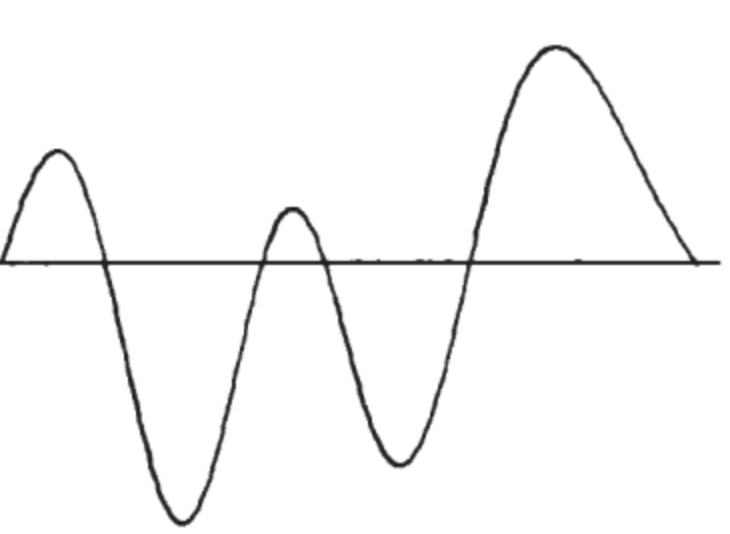
\includegraphics[scale=0.6]{img/SoundSignal.png}
		
			Рис 1.1 — Звуковой сигнал на входе АЦП
\end{center}

\begin{center}
		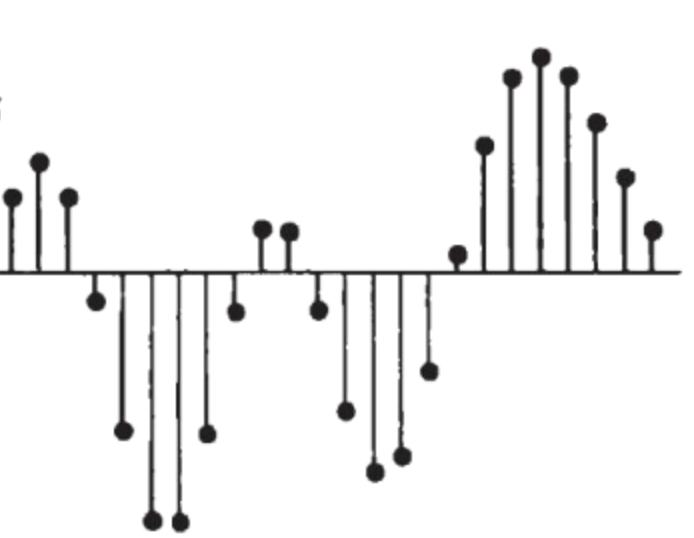
\includegraphics[scale=0.6]{img/DigitalSignal.png}
		
			Рис 1.2 — Дискретный сигнал на выходе АЦП
\end{center} 

Обратное преобразование для воспроизведения звука, закодированного числовым кодом, выполняют цифро-аналоговые преобразователи (ЦАП). 

На рисунках 1.3 и 1.4 представлено обратное преобразование дискретного сигнала в непрерывный звуковой сигнал.

\begin{center}
		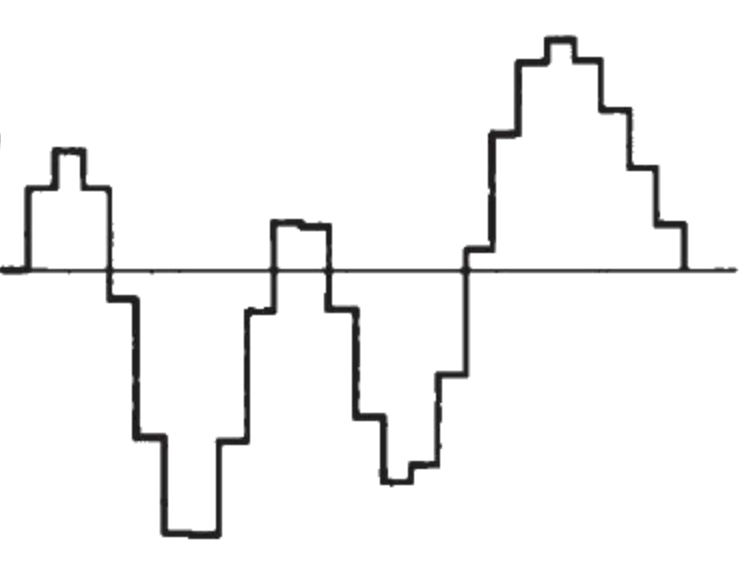
\includegraphics[scale=0.5]{img/DigitalSignal2.png}
		
			Рис 1.3 — Дискретный сигнал на входе ЦАП
\end{center} 

\newpage

\begin{center}
		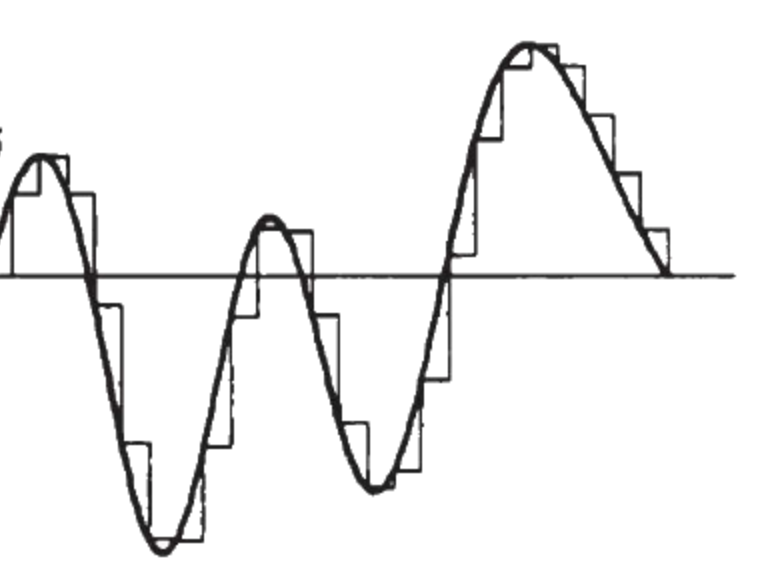
\includegraphics[scale=0.5]{img/SoundSignal2.png}
		
			Рис 1.4 — Звуковой сигнал на выходе ЦАП
\end{center} 

Недостатком данного метода кодирования является то, что синтезированные звуки получаются не слишком похожими на звучание реальных инструментов или других источников закодированного звука.

Таблично-волновой метод (Wave-Table) основан на том, что в заранее подготовленных таблицах хранятся образцы звуков окружающего мира, музыкальных инструментов и так далее. Числовые коды выражают высоту тона, продолжительность и интенсивность звука и прочие параметры, характеризующие особенности звука. Поскольку в качестве образцов используются «реальные» звуки, качество звука, полученного в результате синтеза, получается очень высоким и приближается к качеству звучания реальных музыкальных инструментов \cite{TypesofSynthesis}.

\subsection{Хранение аудиоинформации на компьютере}
Для хранения звуковых данных на компьютере и звуковых носителях в аудиофайлах используются цифровые аудиоформаты. При этом звуковые данные могут быть сжаты для устранения избыточности с помощью устройства или программы, называемой аудиокодеком. Выделяется три основных типа аудиоформатов:
\begin{itemize}
	\item[---]  аудиоформаты без сжатия;
	\item[---]  аудиоформаты со сжатием без потерь;
	\item[---]  аудиоформаты со сжатием с потерями.
\end{itemize}

Некоторые примеры аудиоформатов представлены в таблицах 1 --- 2 \cite{AudioFormats}.

\begin{table}[H]
\caption{Примеры аудиоформатов (часть 1)}
\begin{center}
\begin{tabular}{|p{0.3\linewidth}|p{0.3\linewidth}|p{0.3\linewidth}|}
		\hline
		Расширение & Тип & Описание \\ [0.5ex] 
 		\hline
		 .wav на Windows или .aiff на MAC & Без сжатия & Гибкий аудиоформат, разработанный для хранения любой комбинации частот дискретизации оригинальной звукозаписи. Аудиофайлы с таким форматом достигают большого размера\\
 		\hline MP3 & Сжатие с потерями & Самый популярный аудиоформат. Значительное уменьшение размера данных\linebreak достигается за счет потери качества воспроизведения на профессиональных звуковых системах\\
 		\hline
 		FLAK & Сжатие без потерь & Не нарушает целостность данных, при этом обладая относительной быстротой кодирования/декодирования, гибкостью и средней степенью сжатия\\
		\hline
\end{tabular}
\end{center}
\end{table}

\begin{table}[H]
\caption{Примеры аудиоформатов (часть 2)}
\begin{center}
\begin{tabular}{|p{0.3\linewidth}|p{0.3\linewidth}|p{0.3\linewidth}|}
		\hline
		Расширение & Тип & Описание \\ [0.5ex] 
 		\hline
		AAC & Cжатие с потерями & Преемник MP3 формата с более эффективной компрессией\\
		\hline
		WMA & Сжатие с потерями & Разработан под ОС Windows. Полностью поддерживается Windows, однако при низкой степени сжатия потока качество звука заметно снижается\\
		\hline
		TAK & Cжатие без потерь & При отсутствии потерь в качестве отличается высокой скоростью кодирования/декодирования и степенью сжатия\\
		\hline
		RAW & Без сжатия & Содержит необработанную информацию для обеспечения целостности данных. Не имеет четкой спецификации\\
		\hline
\end{tabular}
\end{center}
\end{table}	

\subsection{MIDI-файлы}

Отдельно от приведенной в таблицах 1.1 -- 1.2 классификации рассматриваются аудиоформаты, содержащие не только оцифрованный звук или не содержащие его вовсе, такие как \textbf{MIDI} формат \cite{AITMAWC}, хранящий наборы инструкций для воспроизведения звука. Аббревиатура MIDI расшифровывается как Musical Instrument Digital Interface (Цифровой интерфейс музыкальных инструментов). Этот формат представляет собой интерфейс музыкальных инструментов, с помощью которого можно кодировать нажатие клавиш, проигрываемые ноты, ссылки на инструменты, значения изменяемых параметров звука и другие данные. Такой способ представления данных позволяет синхронизировать звуковое воспроизведение с управлением различным оборудованием.
При этом последовательность инструкций, хранимая в MIDI-файле, только аппроксимирует нюансы исполнения, игнорируя, например, динамические изменения в продолжительности ноты.
Главной целью разработки такого формата является компактное представление, которое подходит для хранения на дисковом пространстве, но может быть неудобно для хранения в памяти для быстрого доступа \cite{SMFFS}.
Файлы MIDI содержат один или несколько потоков MIDI с информацией о времени для каждого события. Поддерживаются структуры песен и дорожек, информация о темпе и тактовом размере. Названия дорожек и другая описательная информация могут храниться вместе с MIDI-данными. MIDI формат поддерживает несколько дорожек.

MIDI-файлы строятся из фрагментов. Каждый фрагмент имеет 4-символьный тип и 32-битную длину, которая представляет собой количество байтов в фрагменте. Каждый фрагмент начинается с 4-символьного ASCII типа. За ним следует 32-битная длина, старший байт идет первым (например, длина, равная 6 байтам, сохраняется, как 00 00 00 06). Эта длина относится к количеству байтов данных, которые следуют далее: восемь байтов, отведенных для типа и длины, не включены. Таким образом, фрагмент длиной 6 байтов фактически займет 14 байтов дискового пространства.

MIDI-файлы состоят из фрагментов 2-х типов: фрагмент заголовка и фрагмент дорожки. При этом такой файл всегда начинается с фрагмента заголовка, за которым следует один или несколько фрагментов дорожек.

На рисунке 1.5 представлена концепция структуры файла MIDI \cite{SMFFS}.
\begin{center}
		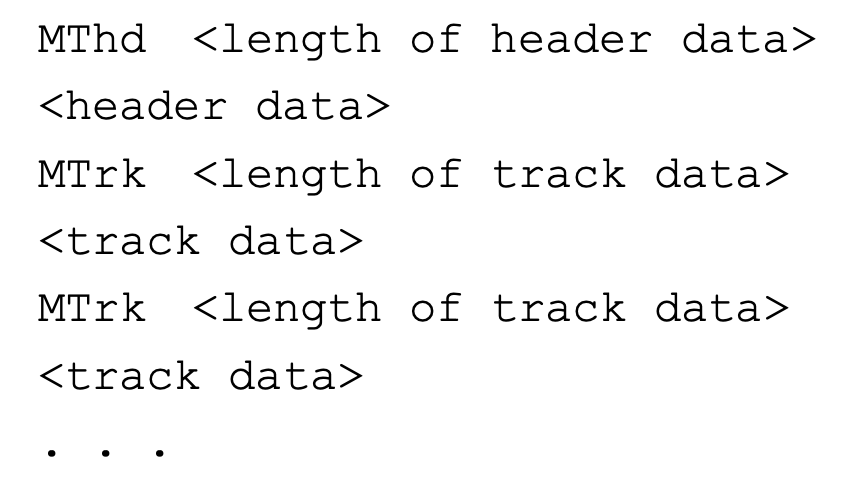
\includegraphics[scale=0.6]{tex/img/MidiStruct.png}
		
			Рис 1.5 — Общая структура файла MIDI
\end{center} 

Фрагмент заголовка предоставляет минимальный объем информации, относящейся ко всему MIDI-файлу и состоит из следующих элементов.
\begin{enumerate}
\item chunk type -- 4-х символьное представление типа фрагмента (MThd).
\item length -- 32-битная величина, значение которой описывает длину в байтах фрагмента без учета первых двух элементов (всегда 6).
\item format -- формат MIDI-файла (2 байта).
\begin{enumerate}
\item 0 -- файл содержит одну единственную дорожку, содержащую MIDI-данные, возможно, для всех 16 каналов. Используется, если секвенсор хранит все  MIDI-данные в одном блоке памяти в том порядке, в котором они воспроизводятся.
\item 1 -- файл содержит одну или несколько одновременных (то есть все начинаются с предполагаемого времени 0) дорожек, возможно, каждая на одном канале. Вместе эти треки считаются одной секвенцией или паттерном. Используется, если  секвенсор разделяет дорожки на разные блоки памяти, но воспроизводит их одновременно.
\item 2 -- файл содержит один или несколько последовательных независимых паттернов, состоящих из одной дорожки. Используется, если секвенсор разделяет дорожки на разные блоки памяти, но воспроизводит только один блок за раз (каждый блок считается отдельным «отрывком» или «песней»).
\end{enumerate}
\item ntrks -- количество дорожек.
\item division -- разрешение, указвающее, как MIDI-тики должны быть переведены во время.
\end{enumerate}

Фрагмент дорожки хранит саму музыкальную информацию и представляет собой поток MIDI-событий (и не MIDI-событий), которому предшествуют значения дельта-времени. 
Каждый такой фрагмент состоит из следуюших элементов.
\begin{enumerate}
\item chunk type -- 4-х символьное представление типа фрагмента (MTrk).
\item length -- 32-битная величина, значение которой описывает длину в байтах фрагмента без учета первых двух элементов.
\item MTrk event -- MIDI- или не MIDI-событие (может быть одно или несколько).
\end{enumerate}

В свою очередь, элемент MTrk event представляется следующими параметрами.
\begin{enumerate}
\item delta-time -- количество времени до следующего события (Если первое событие на дорожке происходит в самом начале дорожки, или если два события происходят одновременно, значение равно 0).
\item event -- либо MIDI-событие (например, такого содержания: идентификатор события, информация о воспроизводимой ноте, ее высоте и положении в октаве и сила извлечения звука), либо не MIDI-событие (события, которые содержат такие данные, как настройки темпа, названия дорожек и тому подобное).
\end{enumerate}

Благодаря такому формату, MIDI-файлы поддерживают хранение музыкальных партитур.
Музыкальная партитура \cite{P} -- это двухмерное представление звуковой последовательности, составляющей музыкальное произведение. Два основных параметра в таком представлении -- это музыкальные ноты, которые должен играть каждый инструмент, и момент, когда звучит каждая нота. Полнофункциональная партитура представляет другие параметры, потому что в партитуру помещается много других элементов, таких как интенсивность каждой ноты и ее изгиб. Тем не менее, два основных параметра достаточны для представления музыки. Таким образом, музыкальная партитура является инструкцией для воспроизведения звука и может храниться в MIDI аудиоформате. Причем в MIDI аудио-файле содержится только одна характеристика: последовательность нот, играемых каждым инструментом, — где ноты имеют начальное сообщение, указывающее на канал (1-16), номер высоты тона в полутонах (1-127), динамику (1-127) и сообщение, свидетельствующее об окончании ноты \cite{AITMAWC}.

Таким образом, MIDI-файлы могут содержать разнообразную информцию о музыке, не ограничиваясь только оцифрованным звуком. При этом формат MIDI разработан так, что даже подробная информация, включающая, например, метаданные и сложные инструкции для воспроизведения нот через различное музыкальное оборудование, имеет компактное представление. Учитывая эти достоинства, дальнейшее рассмотрение аудио-файлов в данной работе ограничивается MIDI форматом, для структуры которого разрабатывается метод распределенного хранения в NoSQL-базе данных.

\clearpage

\section{Существующие решения}

\subsection{Хранение MIDI-файлов в реляционной базе данных PostgreSQL в виде блоба}

\textbf{PostgreSQL} — свободная объектно-реляционная система управления базами данных \cite{PSQL}. 
PostgreSQL предоставляет средства работы с медиафайлами, рассматривающие такие файлы, как большие объекты, или, иначе говоря, блобы (специальный тип данных, предназначенный, в первую очередь, для хранения аудиофайлов и изображений, а также компилированного программного кода) \cite{BLOB}. Механизм больших объектов разбивает данные большого объема на «фрагменты» и сохраняет эти фрагменты в строках таблицы. При произвольном доступе на запись и чтение быстрый поиск нужного фрагмента обеспечивается индексом-B-деревом в этой таблице. Аудиофайлы, записанные в базу данных таким способом, представляются потоком байтов, разбитым на сегменты, каждый из которых не превышает величину LOBLKSIZE (2,05 Кб) для удобного размещения в отдельных строках таблицы \cite{DPSQL}. Потоковый доступ удобен в обработке данных больших объемов, которыми неудобно или невозможно оперировать как одним целым. К тому же это расширяет возможности доступа к отдельным частям данным, что обуславливается механизмом работы со структурой большого объекта: так как данные разбиты на фрагменты, каждый из которых представляет собой кортеж, можно легко получить доступ к любому такому фрагменту без необходимости считывать весь объект. Однако такой подход не позволяет извлечь конкретную часть данных, если не знать структуру хранимого объекта, а именно какой набор байт какой части данных соответствует. Это приводит к тому, что такой способ хранения не подойдет, в случае если необходимо не только хранить и извлекать аудиофайл из базы данных целиком, но и изменять отдельные его части.  

На рисунке 1.6 представлена концептуальня схема хранения MIDI-файлов в базе данных в виде блоба \cite{CBMS}.
\begin{center}
		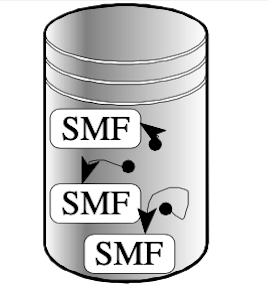
\includegraphics[scale=0.7]{img/blob}
		
			Рис 1.6 — Хранение MIDI-файлов в базе данных в виде блоба
\end{center} 

В PostgreSQL большие объекты хранятся в таблице pg\_largeobject, имеющей следующую структуру (таблица 1.3) \cite{PSQL}.

\begin{table}[H]
\caption{Структура таблицы pg\_largeobject}
\begin{center}
\begin{tabular}{|p{0.3\linewidth}|p{0.3\linewidth}|p{0.3\linewidth}|}
		\hline
		Имя & Тип & Описание \\ [0.5ex] 
 		\hline
		loid & oid & Идентификатор большого объекта, включающего эту страницу\\
		\hline
		pageno & int4 & Номер этой страницы в большом объекте (начиная с 0)\\
		\hline
		data & bytea & Данные, хранящиеся в большом объекте\\
		\hline
\end{tabular}
\end{center}
\end{table}

Для добавления в базу данных большого объекта, сформированного из аудио-файла, существует серверная функция lo\_import(), принимающая путь к файлу на диске. Возвращаемым значением этой функции является идентификатор созданного большого объекта (тип данных oid). Пример добавления содержимого аудио-файла в базу данных PostgreSQL при наличии созданной заранее таблицы audio c атрибутом bigObject\_Id типа oid представлен на листинге \ref{lst:lo_import}.

\newpage

\begin{lstlisting}[language=sql, label=some-code, caption=Пример добавления аудио-файла в базу данных PostgreSQL в виде блоба, label=lst:lo_import]
INSERT INTO audio (bigObjectId)
    VALUES (lo_import("/Users/anastasia/Desktop/ProgramEngineering/audio.mid"));
\end{lstlisting}

В результате, считанные из файла байты, будут добавлены в таблицу pg\_largeobject в виде фрагментов большого объекта. Однако, при таком способе хранения аудио-файла для систем управления базами данных (СУБД) он представляется, как аморфный набор данных, так как СУБД не знает внутренней структуры блоба. Таким образом, операции доступа к конкретным данным MIDI-файла оказываются невозможны.

\subsection{Хранение путей к MIDI-файлу в файловой системе}

Одним из возможных решений хранения аудио-файла в любой базе данных является хранение в базе данных пути к файлу на диске.

На рисунке 1.7 представлена концептуальня схема хранения аудио-файлов в базе данных с использованием пути к файлу \cite{CBMS}.
\begin{center}
		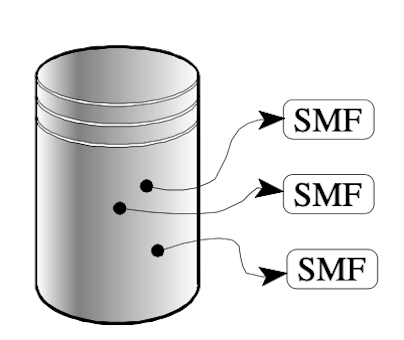
\includegraphics[scale=0.7]{img/disk}
		
			Рис 1.7 — Хранение в базе данных путей к MIDI-файлам, расположенным на дисковом пространстве
\end{center} 

Данный подход не выгоден, так как ответственность за хранилище и расположение файлов в нем полностью делегируется на операционную систему, из-за чего СУБД не может гарантировать целостность набора указателей, а также вся дальнейшая работа с MIDI-файлом предоставляется клиенту, что значительно снижает роль базы данных при таком методе хранения. 

\subsection{Хранение MIDI-файла в виде структуры}

Спецификация MIDI-файлов \cite{SMFFS} позволяет определить внутреннюю структуру аудио-файла, в которой его можно было бы хранить в базе данных. Такой подход удовлетворяет требованию распределенности и возлагает значительную степень ответственности за работу с аудио-информацией на базу данных, освобождая клиента от необходимости использовать дополнительные инструменты, в случае если задача заключается в доступе к определенным элементам структуры MIDI-файла. 

На рисунке 1.8 представлена концептуальня схема хранения аудио-файлов в базе данных на основе их структуры \cite{CBMS}.
\begin{center}
		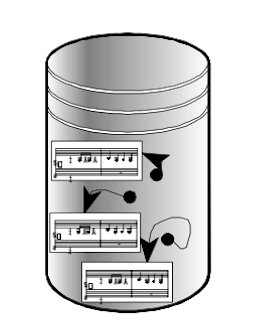
\includegraphics[scale=0.7]{img/musical_scores}
		
			Рис 1.8 — Хранение MIDI-файлов в базе данных на основе их структуры
\end{center} 

Предварительный анализ исходного MIDI-файла в том виде, в котором он хранится на диске, позволит СУБД впоследствии работать со структурированными данными MIDI-файла и, соответственно, отвечать на запросы на основе содержимого хранимой информации, что является наиболее выгодным решением.

\section{Виды существующих NoSQL баз данных}
 \textbf{NoSQL} база данных \cite{WNOSQL} — это база данных, которая не использует реляционную модель данных, а именно организацию хранения данных в виде таблиц и отношений между ними. Вместо этого такие базы ориентированы на какой-то определенный тип данных, под требования хранения которого оптимизируется система хранения таким образом, чтобы процесс запроса был наиболее подходящим для выбранного типа данных. Это позволяет хранить любые данные в NoSQL базах нерегламентированно (гибкость модели данных), а также размещать данные большого объема с относительно быстрым доступом к ним за счет масштабируемости. Главное правило проектирования структуры данных в NoSQL базах — она должна подчиняться требованиям приложения и быть максимально оптимизированной под наиболее частые запросы. Термин "NoSQL" расшифровывается как "Not Only SQL" и, подразумевая под собой ответвление SQL-подхода к проектированию баз данных, является собирательным определением альтернатив к организации хранения и доступа к данным средствами SQL. 
 
 По модели данных NoSQL-базы данных классифицируются на следующие основные виды.
\begin{enumerate}
\item Ключ — значение.
\item Документы.
\item Семейства столбцов.
\item Графы.
\end{enumerate}

 В таблицах 1.4 --- 1.6 представлена сравнительная характеристика баз данных SQL и NoSQL \cite{AMNOSQL}.

\clearpage 

\begin{table}[h]
\caption{Сравнительная характеристика баз данных SQL и NoSQL (часть 1)}
\begin{center}
\begin{tabular}{|l|p{0.25\linewidth}|p{0.41\linewidth}|p{0.35\linewidth}|}
		\hline
		Критерий/Тип БД & Реляционные & NoSQL \\ [0.5ex] 
 		\hline
		 Модель данных & Используют реляционную модель, которая преобразует данные в двумерные таблицы, состоящие из строк и столбцов & Используют разнообразные модели данных, такие как пары «ключ-значение», документы и графы, оптимизированные под определенный тип хранимых даных для высокой производительности и горизонтальной масштабируемости\\
 		\hline 
		Схема данных & Схема жестко задает таблицы, строки, столбцы, индексы, отношения между таблицами и прочие элементы базы данных. Такая БД обеспечивает целостность ссылочных данных в отношениях между таблицами. & Гибкая схема\\
 		\hline
 \end{tabular}
\end{center}
\end{table}

\clearpage

\begin{table}[h]
\caption{Сравнительная характеристика баз данных SQL и NoSQL (часть 2)}
\begin{center}
\begin{tabular}{|l|p{0.25\linewidth}|p{0.41\linewidth}|p{0.35\linewidth}|}
		\hline
		Критерий/Тип БД & Реляционные & NoSQL \\ [0.5ex] 
		\hline
		Выполнение запросов & Запросы составляются на языке SQL. Эти запросы анализирует и выполняет реляционная база данных & Для записи/извлечения могут использоваться объектно-ориентированные API. Поиск может осуществляться по парам «ключ-значение», наборам столбцов и т. д.\\
		\hline
		Масштабирование & Обычно масштабируются путем увеличения вычислительных возможностей аппаратного обеспечения или добавления отдельных копий для рабочих нагрузок чтения (преимущественно вертикальное масштабирование) & Обычно поддерживают высокую разделяемость благодаря шаблонам доступа с возможностью масштабирования на основе распределенной архитектуры. Это повышает пропускную способность и обеспечивает устойчивую производительность почти в неограниченных масштабах (горизонтальное масштабирование)\\
		\hline
\end{tabular}
\end{center}
\end{table}

\clearpage

\begin{table}[h]
\caption{Сравнительная характеристика баз данных SQL и NoSQL (часть 3)}
\begin{center}
\begin{tabular}{|l|p{0.25\linewidth}|p{0.41\linewidth}|p{0.35\linewidth}|}
		\hline
		Критерий/Тип БД & Реляционные & NoSQL \\ [0.5ex] 
 		\hline
 		Производительность & Производительность главным образом зависит от дисковой подсистемы. Для обеспечения максимальной производительности часто требуется оптимизация запросов, индексов и структуры таблицы. & Производительность обычно зависит от размера кластера базового аппаратного обеспечения, задержки сети и вызывающего приложения\\
 		\hline
\end{tabular}
\end{center}
\end{table}

\clearpage

\subsection{Модель данных Ключ-Значение}

Модель данных, реализующяя хранение по типу ключ‑значение связывает каждое значение данных с уникальным ключом. Большинство СУБД с такой моделью данных поддерживают только самые простые операции запроса, вставки и удаления, а также, как правило, используют хеш-таблицу, в которой находится уникальный ключ и указатель на конкретный объект данных. Производительность сильно вырастает за счёт кеширующих механизмов. 
Как ключи, так и значения могут представлять собой что угодно: от простых до сложных составных объектов. Базы данных с использованием пар ключ‑значение поддерживают высокую разделяемость и обеспечивают беспрецедентное горизонтальное масштабирование, недостижимое при использовании других типов баз данных. Однако, чтобы частично или полностью изменить значение, приложение всегда перезаписывает существующее значение целиком. Также СУБД, имеющие такую модель данных, не оптимизированы для запросов по значению.

\subsection{Модель данных документов}

Документоориентированная модель данных хранит данные, представленные парами ключ-значение, которые сжимаются в виде полуструктурированного документа из тегированных элементов, подобно JSON, XML, BSON и другим подобным форматам. В базе данных документов хранится коллекция документов, в которой каждый документ состоит из именованных полей и данных. Данные могут быть простыми значениями или сложными элементами, такими как списки и дочерние коллекции. Документы извлекаются по уникальным ключам. 

Одним из ключевых различий между моделью данных по типу ключ-значение и документоориентированным хранением является то, что последнее включает метаданные, связанные с хранимым содержимым, что даёт возможность делать запросы на основе содержимого. Тот факт, что такие базы данных работают без схемы, делает простой задачей добавление полей в документы без необходимости сначала заявлять об изменениях. 

Документные базы данных позволяют разработчикам хранить и запрашивать данные в БД с помощью той же документной модели, которую они используют в коде приложения. Гибкий, полуструктурированный, иерархический характер документов и документных баз данных позволяет им развиваться в соответствии с потребностями приложений.Документные базы данных обеспечивают гибкость индексации, производительность выполнения стандартных запросов и аналитику наборов документов.

\subsection{Модель данных семейства столбцов}

В колоночных NoSQL-базах данных данные хранятся в ячейках, сгруппированных в колонки, а не в строки данных. Колонки логически группируются в колоночные семейства. Колоночные семейства могут состоять из практически неограниченного количества колонок, которые могут создаваться во время работы программы или во время определения схемы. Чтение и запись происходит с использованием колонок, а не строк.

В сравнении с хранением данных в строках, как в большинстве реляционных баз данных, преимущества хранения в колонках заключаются в быстром поиске/доступе и агрегации данных. Реляционные базы данных хранят каждую строку как непрерывную запись на диске. Разные строки хранятся в разных местах на диске, в то время как колоночные базы данных хранят все ячейки, относящиеся к колонке, как непрерывную запись, что делает операции поиска/доступа быстрее.

В отличие от модели данных на основе пар ключ-значение и модели данных документов, большинство хранилищ столбцов используют для упорядоченного хранения данных сами значения ключей, а не хеш-коды от них. Многие реализации позволяют создавать индексы по определенным столбцам в семействе столбцов. Индексы позволяют получать данные по значениям столбцов, а не ключам строки. 

\subsection{Модель данных графов}

В графовой базе данных нет строгого формата SQL или представления таблиц и колонок, вместо этого используется гибкое графическое представление, которое подходит для решения проблем масштабируемости. База данных графов хранит сведения двух типов: узлы и грани. Ребра задают связи между узлами. Узлы и ребра могут иметь свойства, предоставляющие сведения об этом узле или ребра, аналогичные столбцам в таблице. Грани могут иметь направление, указывающее на характер связи. Обход графа в графовой базе данных можно выполнять либо по определенным типам ребер, либо по всему графу. Обход соединений или взаимосвязей в графовых базах данных выполняется очень быстро, поскольку взаимосвязи между узлами не вычисляются во время выполнения запроса, а хранятся в базе данных. Тем не менее, модель данных графов отличается высокой сложностью реализации.

\subsection{MongoDB}

MongoDB  \cite{Mongo} -- система управления базами данных, которая работает с документоориентированной моделью данных и для хранения данных использует формат, подобный JSON \cite{JSON}, -- формат BSON \cite{BSON}. Данный формат представляет собой двоично-кодированную сериализацию JSON-подобных документов. Как и JSON, BSON поддерживает встраивание документов и массивов в другие документы и массивы. BSON также содержит расширения, позволяющие представлять типы данных, не входящие в спецификацию JSON. Например, BSON имеет тип BinData \cite{BinData}.

Данные в BSON-формате хранятся в документах, которые хранятся в коллекции. Это означает, что структура сохраняемых данных может быть изменена для каждой записи и не требуется, чтобы она соответствовала предварительно определенному шаблону. Хранилище в BSON-формате также позволяет вкладывать данные, благодаря чему можно хранить сложноорганизованные данные с любой структурой. MongoDB поддерживает поиск по полям, диапазонные запросы и поиск по регулярным выражениям. Могут быть сделаны запросы для возврата определенных полей в документах. Также MongoDB использует концепцию шардинга для горизонтального масштабирования с помощью разделения данных между несколькими экземплярами БД. Она может работать на нескольких серверах, балансируя нагрузку и/или дублируя данные, чтобы поддерживать работоспособность системы в случае аппаратного сбоя. 

Терминология MongoDB отличается от терминологии SQL. Основные понятия баз данных сопоставлены в таблице 1.7.

\begin{table}[H]
\caption{Сравнение терминологии MongoDB и терминологии SQL}
\begin{center}
\begin{tabular}{|p{0.3\linewidth}|p{0.3\linewidth}|}
		\hline
		MongoDB & SQL \\ [0.5ex] 
 		\hline
		Коллекция & Таблица \\
		\hline
		Документ & Ряд \\
		\hline
		Поле & Столбец \\
		\hline
		ObjectId & Первичный ключ \\
		\hline
\end{tabular}
\end{center}
\end{table}

\section{Выбор NoSQL-базы данных}

В качестве NoSQL-базы данных, наиболее подходящей под хранение аудио-файлов формата MIDI на основе их структуры, была выбрана база данных MongoDB, так как она является свободной и одной из самых распространенных документоориентированных баз данных. Это означает, что структура сохраняемых данных может быть изменена для каждой записи в базу и не требует, чтобы она была в предварительно определенном формате. Хранилище в формате BSON, отличающемся гибкой структурой, высокой скоростью сканирования и кодирования и декодирования данных, а также наличием типов данных, не поддерживаемых форматом JSON, позволяет вкладывать данные, что особенно важно для хранения аудио-файлов в MIDI формате, содержащих произвольное количество музыкальных дорожек. Возможность хранения разных типов данных в непредопределенной стрктуре позволяет хранить музыкальные данные в любом формате, адаптируемом под бизнес-требования. В частности, такой тип, как "бинарные данные" (BinData), очень удобен для представления некоторых элементов MIDI-файлов, например, для массива байтов, отвечающих за MIDI- и не Midi-события во фрагменте музыкальной дорожки. Помимо этого, MongoDB предоставляет возможности репликации и ограниченную поддержку шардинга, что обеспечивает высокие доступность и надежность и балансировку нагрузки. Также у MongoDB есть клиентские библиотеки для основных языков программирования, таких как C \cite{C}, C++ \cite{CPP}, C\# \cite{CS}, Python \cite{Python}, Java \cite{Java} и других. Открытый исходный код предоставляет возможность изучить внутреннее устройство СУБД и разработать программное обеспечение, которое впоследствии может быть интегрировано в систему.

\subsection{Выводы из аналитического раздела}

В данном разделе были приведены теоретические сведения о звуковой информации, об аудио-форматах и о существующих NoSQL-базах данных, а также были рассмотрены способы хранения аудио-файлов в базе данных. Было выяснено, что наиболее полноценную и разнородную информацию содержат аудио-файлы формата MIDI, которые наиболее оптимально хранить на основе их внутренней структуры. Также была приведена сравнительная характеристика реляционных и NoSQL-баз данных и сравнительная характеристика видов нереляционных баз данных по модели данных. На основе полученного сравнительного анализа, было установлено, что наиболее подходящим решением для хранения MIDI-файлов на основе их структуры является хранение в документоориентированной NoSQL-базе данных MongoDB.

\clearpage


%%% Local Variables:
%%% mode: latex
%%% TeX-master: "rpz"
%%% End:

\chapter{Конструкторский раздел}
\label{cha:design}

\section{Основные операции для работы с данными}

Разработанный метод распределенного хранения аудио-файлов в NoSQL-базе данных применяется на этапах добавления и извлечения аудио-файла из базы данных. 

\subsection{Добавление аудио-файла в MongoDB}

В процессе обработки операции записи данных в базу данных выполняется валидация глубины документа и проверка на наличие заданного клиентом идентификатора, а такаже присвоение идентификатора, в случае если его нет. Разработанный метод применяется на этом же уровне и состоит из следующих шагов.
\begin{enumerate}
\item Прверка на то, что данные являются MIDI-файлом (данные должны соответствовать определенной структуре, а также аудио-файл должен существовать и являться MIDI-файлом).
\item Извлечение пути к аудио-файлу и его имени для дальнейшего извлечения
\item Считывание содержимого аудио-файла.
\item Создание документа со специальной структурой (Parser).
\end{enumerate}

На рисунке 2.1 представлена функциональная декомпозиция этапов добавления аудио-файла в MongoDB.

\begin{center}
		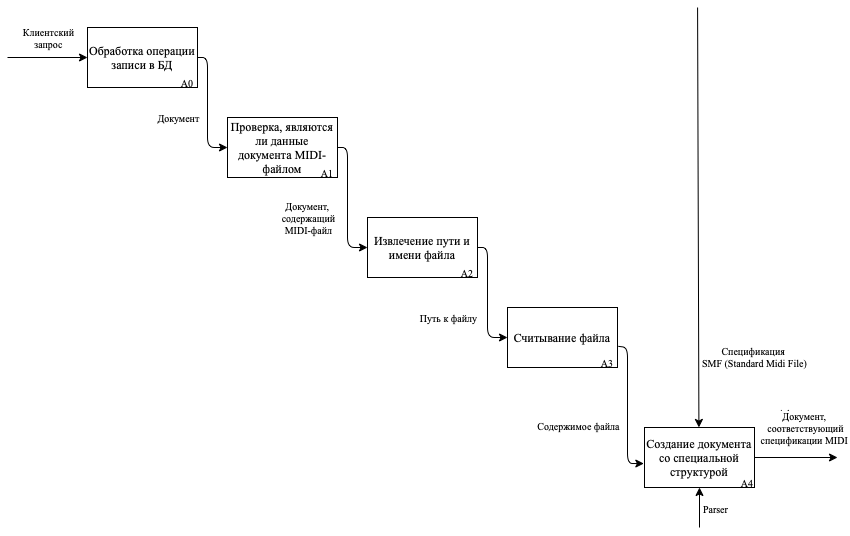
\includegraphics[scale=0.55]{tex/img/DecomposeInsert1.png}
		
			Рис 2.1 — Функциональная декомпозиция этапов добавления аудио-файла в MongoDB
\end{center} 

Формирование специальной структуры, соответствующей спецификации MIDI-файла, выполняется с помощью метода, представленного на листингах \ref{lst:parser_midi1} -- \ref{lst:parser_midi3}. Так как данные в MongoDB хранятся в виде объектов типа BsonDocument, весь MIDI-файл представлен в виде такого документа, где каждое поле является либо объектом типа BsonElement, либо, если имеет несколько полей, подобъектом типа BsonDocument, либо массивом подобъектов.

Тип BsonElement имеют следующие элементы MIDI-файла.

\begin{enumerate}
\item ID -- идентификатор заголовка MIDI (MThd) или музыкальной дорожки (MTrk). Тип данных: строка.
\item Length -- длина фрагмента заголовка или фрагмента музыкальной дорожки. Тип данных: бинарные данные.
\item Format -- формат MIDI-файла. Тип данных: бинарные данные.
\item NumTracks -- количество музыкальных дорожек. Тип данных: бинарные данные.
\item Devision -- разрешение MIDI-файла. Тип данных: бинарные данные.
\item Data -- данные музыкальной дорожки. Тип данных: бинарные данные.
\end{enumerate}
 
Также структура документа MongoDB, содержащего аудио-файл, была дополнена еще одним объектом типа BsonElement -- Name -- имя MIDI-файла, используемое при извлечении из базы данныхс опцией сохранения на диске. Тип данных: строка.

Тип BsonArray имеет поле <<MTrks>>, содержащее список объектов BsonDocument (каждый объект представляет одну музыкальную дорожку).

На рисунках 2.2 -- 2.5  представлена схема метода создания документа MongoDB по спецификации MIDI.

\begin{center}
		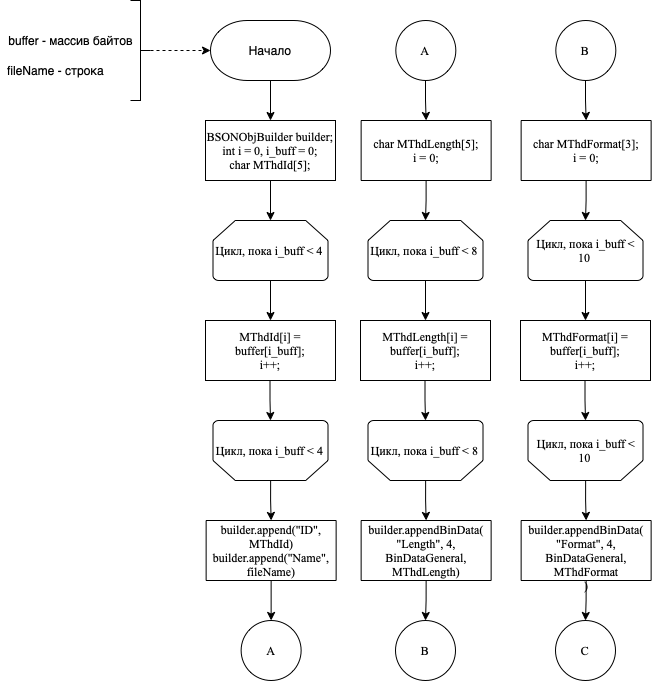
\includegraphics[scale=0.7]{tex/img/Parser1.png}
		
			Рис 2.2 — Схема метода создания документа MongoDB по спецификации MIDI (часть 1)
\end{center}

\begin{center}
		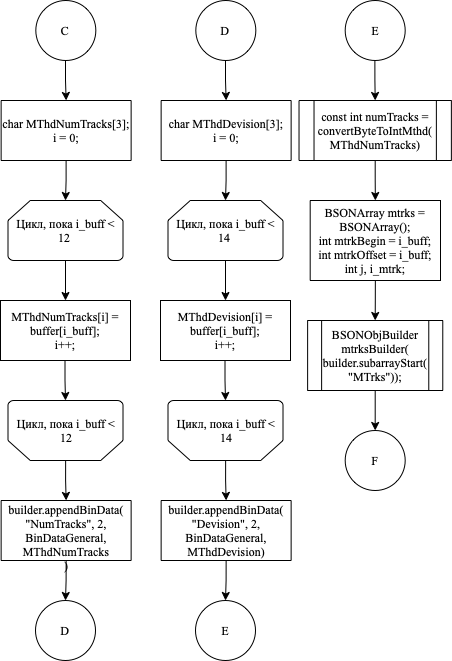
\includegraphics[scale=0.7]{tex/img/Parser2_1.png}
		
			Рис 2.3 — Схема метода создания документа MongoDB по спецификации MIDI (часть 2)
\end{center}

\begin{center}
		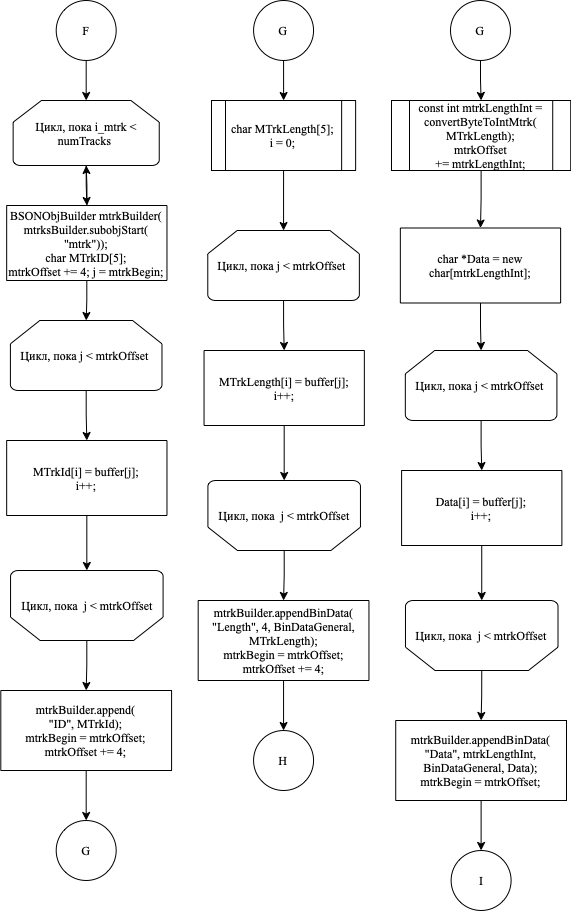
\includegraphics[scale=0.7]{tex/img/Parser3_1.png}
		
			Рис 2.4 — Схема метода создания документа MongoDB по спецификации MIDI (часть 3)
\end{center}

\begin{center}
		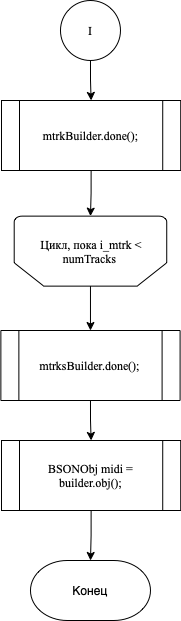
\includegraphics[scale=0.7]{tex/img/Parser4-2.png}
		
			Рис 2.5 — Схема метода создания документа MongoDB по спецификации MIDI (часть 4)
\end{center}

\subsection{Извлечение аудио-файла из MongoDB}

В ходе выполнения операции извлечения документа или набора документов из базы данных записи, содержащие MIDI-информацию, обрабатываются особым образом. Извлечение документа, имеющего структуру MIDI-файла, дополняется опцией сохранения данных локально в виде аудио-файла. После того как к запросу на извлечение данных применяется парсинг системы, извлекающий данные запроса, выполняется извлечение фильтра запроса и проверяется наличие в нем поля MidiSave, являющегося флагом, сигнализирующим о желании пользователя сохранить струкутуру MIDI-файла локально в формате аудио-файла с расширением <<.mid>>. Затем, когда запрос будет выполнен, в случае если в фильтре запроса есть поле MidiSave и оно имеет значение True, сохранение метода осуществится в три этапа.
\begin{enumerate}
\item Прверка на то, что данные являются MIDI-файлом (данные должны
соответствовать определенной структуре).
\item Формирование массива байтов из документа.
\item Запись массива байтов в файл.
\end{enumerate}

На рисунке 2.6 представлена функциональная декомпозиция этапов извлечения аудио-файла из MongoDB (если документ MongoDB необходимо сохранить в виде аудио-файла).

\begin{center}
		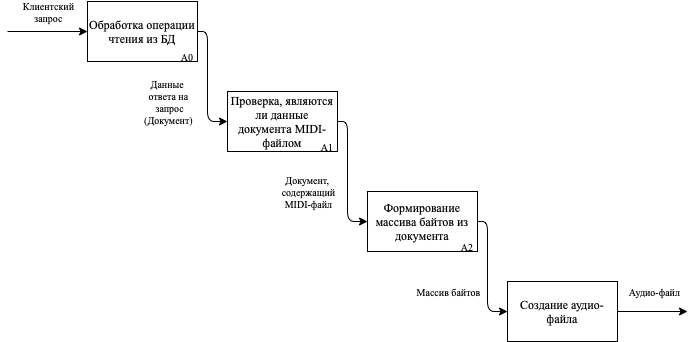
\includegraphics[scale=0.55]{tex/img/DecomposeFind.png}
		
			Рис 2.6 — Функциональная декомпозиция этапов извлечения аудио-файла из MongoDB (в случае записи документа MongoDB на диск в виде аудио-файла)
\end{center} 

Если в фильтре запроса нет поля MidiSave или оно имеет значение False, документ MongoDB не будет представлен в виде MIDI-файла и будет только возвращен клиенту в стандратном виде BsonDocument.

На рисунках 2.7 -- 2.9  представлена схема метода воссоздания MIDI-файла из документа MongoDB (листинги \ref{lst:file_builder1} -- \ref{lst:file_builder2}).

\begin{center}
		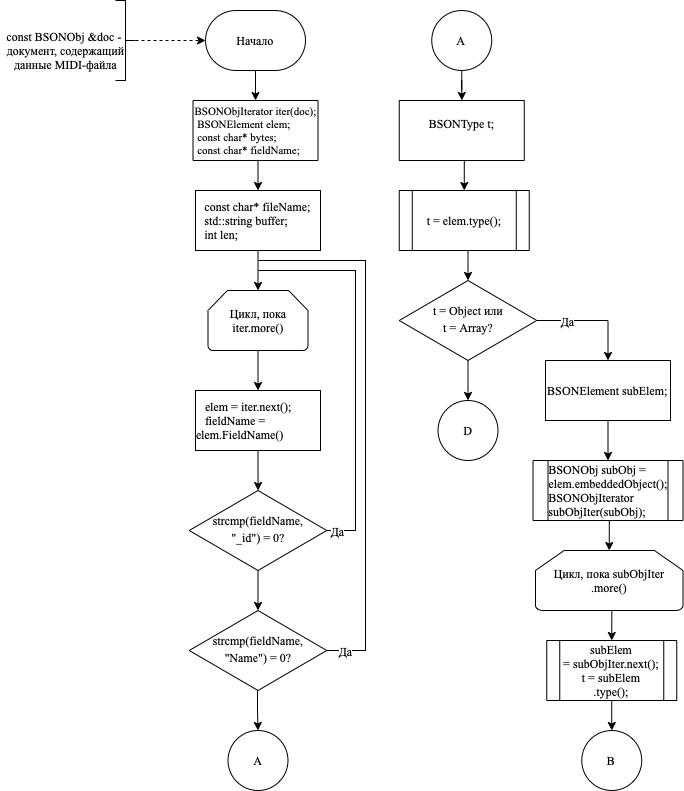
\includegraphics[scale=0.65]{tex/img/FileBuilder1.png}
		
			Рис 2.7 — Схема метода воссоздания MIDI-файла из документа MongoDB (часть 1)
\end{center}

\begin{center}
		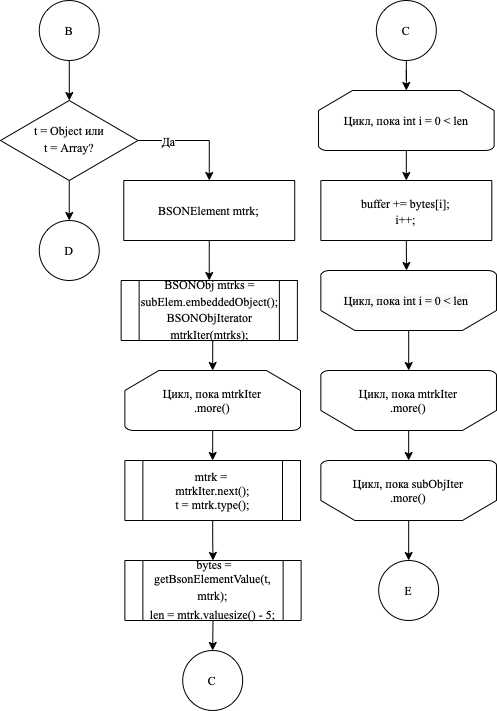
\includegraphics[scale=0.7]{tex/img/FileBuilder2.png}
		
			Рис 2.8 — Схема метода воссоздания MIDI-файла из документа MongoDB (часть 2)
\end{center}

\begin{center}
		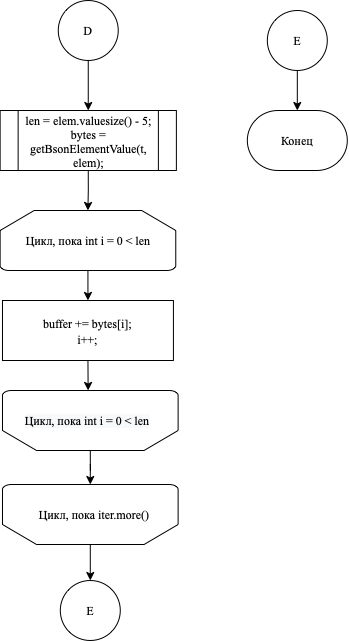
\includegraphics[scale=0.7]{tex/img/FileBuilder3.png}
		
			Рис 2.9 — Схема метода воссоздания MIDI-файла из документа MongoDB (часть 3)
\end{center}

\section{Ограничения предметной области}

Ограничения предметной области включают следующие пункты.

\begin{enumerate}
\item Добавление MIDI-файла в MongoDB и извлечение документа с его последующей записью на диск в формате MIDI-файла имеют жестко заданные API.
\begin{enumerate}
\item API записи аудио-файла в базу данных включает в себя все команды вставки, но имеет строгую структуру, представленную на листинге \ref{lst:insert_structure}, где path -- это путь к аудио-файлу, а name (может быть опущено) -- имя файла, используемое при сохранении документа в формате MIDI файла. Если эта структура не будет соблюдена, вставки аудио-файла в базу в предусмотренном в разработанном методе формате не произойдет.
\item API чтения аудио-файла из базы данных включает в себя все команды чтения, но для сохранения документа в виде аудио-файла необходимо задать поле MidiSave фильтра запроса, установив ему значение True.
\end{enumerate}
\item Пользователь не имеет возможности задавать тип данных, в котором будут храниться поля аудио-файла в базе данных.
\item Данные, представляющие музыкальную дорожку, не разбиваются на логические подструктуры.
\end{enumerate}

\begin{lstlisting}[language=C, label=some-code, caption=Структура запроса на добавление аудио-файла в MongoDB, label=lst:insert_structure]
{ 
    path: string("some data"),
    name: string("some data")
}
\end{lstlisting}

\section{Выводы из конструкторского раздела}

В данном разделе были описаны основные операции для работы с данными при использовании разработанного метода распределенного хранения аудио-файлов в NoSQL-базе данных, была проведена функциональная декомпозиция этих операций, были представлены схемы работы метода, реализующего создание документа MongoDB, соответствующего спецификации MIDI, из сырого содержимого аудио-файла. Также были определены ограничения предметной облвсти.
%%% Local Variables:

%%% mode: latex
%%% TeX-master: "rpz"
%%% End:
%--количество цветов
%||количество пикселей
\chapter{Технологический раздел}

\section{Выбор языка программирования}

В качестве языка программирования был выбран C++, так как на нем написана серверная часть базы данных MongoDB. Соответственно, метод хранения аудио-файлов для MongoDB был разработан, как патч для действующей версии СУБД.

\section{Выбор среды разработки}

Для программной реализации метода был выбран редактор кода Visual Studio Code \cite{VSC}, так как он обладает следующими достоинствами.
\begin{enumerate}
\item Кроссплатформенность.
\item Поддержка большого набора языков программирования, включая C++.
\item Широкие возможности кастомизации.
\item Открытый исходный код.
\end{enumerate}

\section{Выбор инструментов для замеров времени}

Для доступа к базе данных использовался драйвер C\# для MongoDB -- MongoDB.Driver \cite{CSDriver}, обеспечивающий асинхронное взаимодействие с MongoDB. MongoDB.Driver предоставляет API для подключения к серверу базы данных и выполнения запросов любой сложности через клиента. Такой подход наиболее удобен, когда планируется последующая программная обработка данных, как в случае с замером времени работы с данными при выбранном методе хранения.
Программное обеспечение было реализовано в интегрированной среде разработки Rider \cite{Rider}, которая является кроссплатформенной, предоставляет удобные и быстрые редактор кода и отладчик, поддерживает платформу .Net \cite{Net} для создания приложений на языке C\#, а также имеет свободный доступ для студентов. Установка драйвера была произведена с помощью пакетного менеджера NuGet \cite{NuGet}, имеющего удобный интерфейс в среде Rider, и была интегрирована в сборку проекта с помощью системы управления зависимостями .Net с указанием версии используемого пакета. На рис. 1.1 представлен фрагмент сборки приложения с драйвером MongoDB.Driver.

\begin{center}
		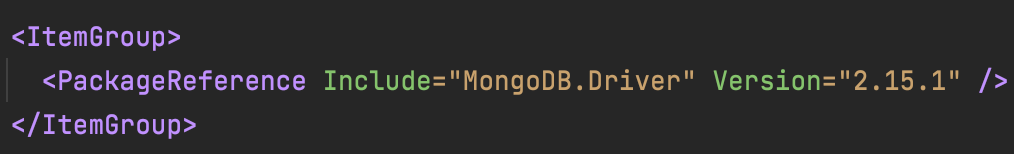
\includegraphics[scale=0.6]{img/MongoDriver}
		
			Рис 1.1 — Фрагмент сборки .Net приложения с интеграцией драйвера MongoDB.Driver 
\end{center} 

Для замеров времени работы реализованного метода при тестировании и сравнении его с аналогом хранения использовалась бибилиотека BenchmarkDotNet \cite{BenchMark}. BenchmarkDotNet - это легкая и мощная библиотека .NET с открытым исходным кодом, которая может преобразовывать методы в тесты, отслеживать эти методы, а затем предоставлять анализ полученных данных о производительности. BenchmarkDotNet обеспечивает высокую точность полученных результатов благодаря использованию набора инструментов для анализа производительности Perfolizer \cite{Perfolizer}. Широкий спектр возможностей, которые предоставляет данная библиотека, включает в себя анализ тестов, предупреждающий ошибки, и экспорт результатов сравнительного анализа методов в необходимом пользователю формате. Результатом запуска метода Run() данного инструмента со стандартной конфигурацией будет сводная таблица показателей производительности тестируемых методов.
BenchmarkDotNet была установлена в среду разработки так же с помощью менеджера пакетов NuGet и интегрирована в сборку проекта системой управления зависимостями. На рис. 1.2 представлен фрагмент сборки приложения с библиотекой BenchmarkDotNet.

\begin{center}
		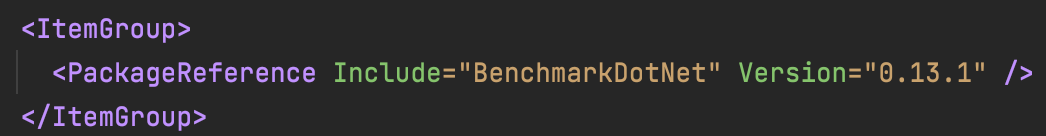
\includegraphics[scale=0.6]{img/BenchmarkDotNet}
		
			Рис 1.2 — Фрагмент сборки .Net приложения с интеграцией библиотеки BenchmarkDotNet 
\end{center} 

\section{Сборка локального сервера MongoDB}

Следуя инструкции по сборке MongoDB из исходного кода, расположенной в официальном репозитории базы данных \cite{Instruction}, для компиляции сервера MongoDB использовался инструмент для автоматизации сборки программных проектов SCons \cite{SCons}. Команда, использовавшаяся для запуска компиляции сервера MongoDB в командной строке с помощью SCons, представлена в листинге \ref{lst:scons_command}, где 
\begin{enumerate}
\item dbg -- вывод отладочной информации.
\item j8 -- количество логических ядер, между которыми распределяется нагрузка при компиляции (8).
\item install-mongod -- цель, указывающая какой компонент нужно скомпилировать.
\end{enumerate}

\begin{lstlisting}[language=sql, label=some-code, caption=Команда для компиляции сервера MongoDB средствами SCons, label=lst:scons_command]
sudo scons --dbg -j8 install-mongod  
\end{lstlisting}

Для сборки SCons использует скрипты SConstruct, расположенные в файловой структуре проекта, одними из задач которых является импортирование необходимых модулей Python и проверка инструментов, участвующих в компиляции, на соответствие требованиям.

Для успешной сборки определены следующие требования.

\begin{enumerate}
\item Современный С++ компилятор. Подходят следующие компиляторы.
\begin{enumerate}
\item G++ 8.2 \cite{GCC} или новее.
\item Clang 7.0 \cite{Clang} или новее.
\end{enumerate}
\item В операционных системах Linux \cite{Linux} и macOS \cite{macOS} требуется библиотека и заголовок libcurl \cite{LibCurl}. MacOS включает libcurl.
\item Python 3.7 и некоторые модули, устанавливаемые с помощью команды, представленной в листинге \ref{lst:python_modules}.
\item Около 13 ГБ свободного места на диске для скомпилированных двоичных файлов.
\end{enumerate}

\begin{lstlisting}[language=sql, label=some-code, caption=Команда для установки необходимых для сборки модулей Python, label=lst:python_modules]
python3 -m pip install -r etc/pip/compile-requirements.txt  
\end{lstlisting}

SCons также предоставляет возможность скомпилировать отдельные компоненты MongoDB, задав одну или несколько из следующих целей.
\begin{enumerate}
\item install-mongod -- сервер базы данных.
\item install-mongos -- шардинг.
\item install-servers -- включает install-mongod и install-mongos.
\item install-core -- включает install-mongod и install-mongos.
\item install-mongosh -- полнофукционольная среда для взаимодействия с развертываниями MongoDB, использующая интерфейс командной строки.
\item install-all -- все компоненты.
\end{enumerate}

\section{Структура проекта}

В проект базы данных MongoDB было добавлено два исходных файла, реализующих логику добавления и извлечения MIDI-файла, а также заголовочные файлы для них. 

Так как MIDI-файл, в соответствии с разработанным методом, хранится в виде предварительно распарсенной структуры, программный код, выполняющий считывание потока байтов из файла и конструирование из него документа, находится в части проекта, отвечающей за выполнение операции вставки в базу данных. На этапе валидирования добавляемого документа выполняется проверка на то, содержит ли он путь к MIDI-файлу, и если да -- документ пересобирается с использованием парсера, чтобы впоследствии представлять внутреннюю структуру аудио-файла.

В проект по пути src/mongo/db/ops/ были добавлены следующие файлы для парсинга MIDI-файла на этапе вставки документа в MongoDB.
\begin{enumerate}
\item insert\_midi.cpp -- исходный файл, реализующий чтение MIDI-файла и парсер.
\item insert\_midi.h -- заголовочный файл.
\end{enumerate}

Для дальнейшей работы с добавленным документом, как с аудио-файлом, предусмотрено обратное преобразование структуры в MIDI-файл в процессе извлечения документы из базы данных. Для этого добавлена проверка на то, что запись в MongoDB является MIDI-файлом, и последовательная запись данных в файл с именем, которое было указано пользователем в качестве второго поля при вставке аудио-файла (name) или, в случае если пользователь указал только путь к файлу, извлечено из пути.

В проект по пути src/mongo/db/commands/ были добавлены следующие файлы для воссоздания MIDI-файла на этапе извлечения документа из MongoDB.
\begin{enumerate}
\item find\_midi.cpp -- исходный файл, реализующий обратное преобразование документа в MIDI-файл.
\item find\_midi.h -- заголовочный файл.
\end{enumerate}

Для успешной сборки проекта после добавления новых файлов требуется указать их в конфигурации соответствующих файлов SConstruct. Следовательно, были изменены следующие скрипты.
\begin{enumerate}
\item src/mongo/db/SConscript.
\item src/mongo/db/commands/SConscript.
\end{enumerate}

\section{Пример работы реализованного метода}

Для демонстрации работы метода был создан клиент MongoDB на языке Python с помощью библиотеки pymongo \cite{PyMongo}. Помимо поддержки API доступа к MongoDB и работы с ней, Python предоставляет возможность загружать и проигрывать аудиозаписи различных форматов, как фоновую музыку, с использованием средств библиотеки pygame \cite{PyGame}. Также Python содержит бибилиотеку tkinter \cite{Tk}, с помощью которой был реализован простой графический интерфейс для удобства работы с базой данных.

Однако, независимо от используемого клиента, структура данных для запроса на добавление MIDI-файла в базу данных примет следующий вид (листинг \ref{lst:insert_command}).

\begin{lstlisting}[language=sql, label=some-code, caption=Данные для запроса на добавление MIDI-файла в MongoDB, label=lst:insert_command]
{path: "/Users/anastasia/Desktop/ProgramEngineering/some_audio.mid",  name:"my_audio"}
\end{lstlisting}

Для извлечения данных с последующим сохранением MIDI-файла с названием my \_audio достаточно установить в фильтре запроса на извлечение значение True поля MidiSave. Если не нужно сохранять аудио-файл локально, значение поля MidiSave в фильтре можно установить равным False или опустить.

На рисунке 1.3 представлен реализованный для демонстрации графический интерфейс.

\begin{center}
		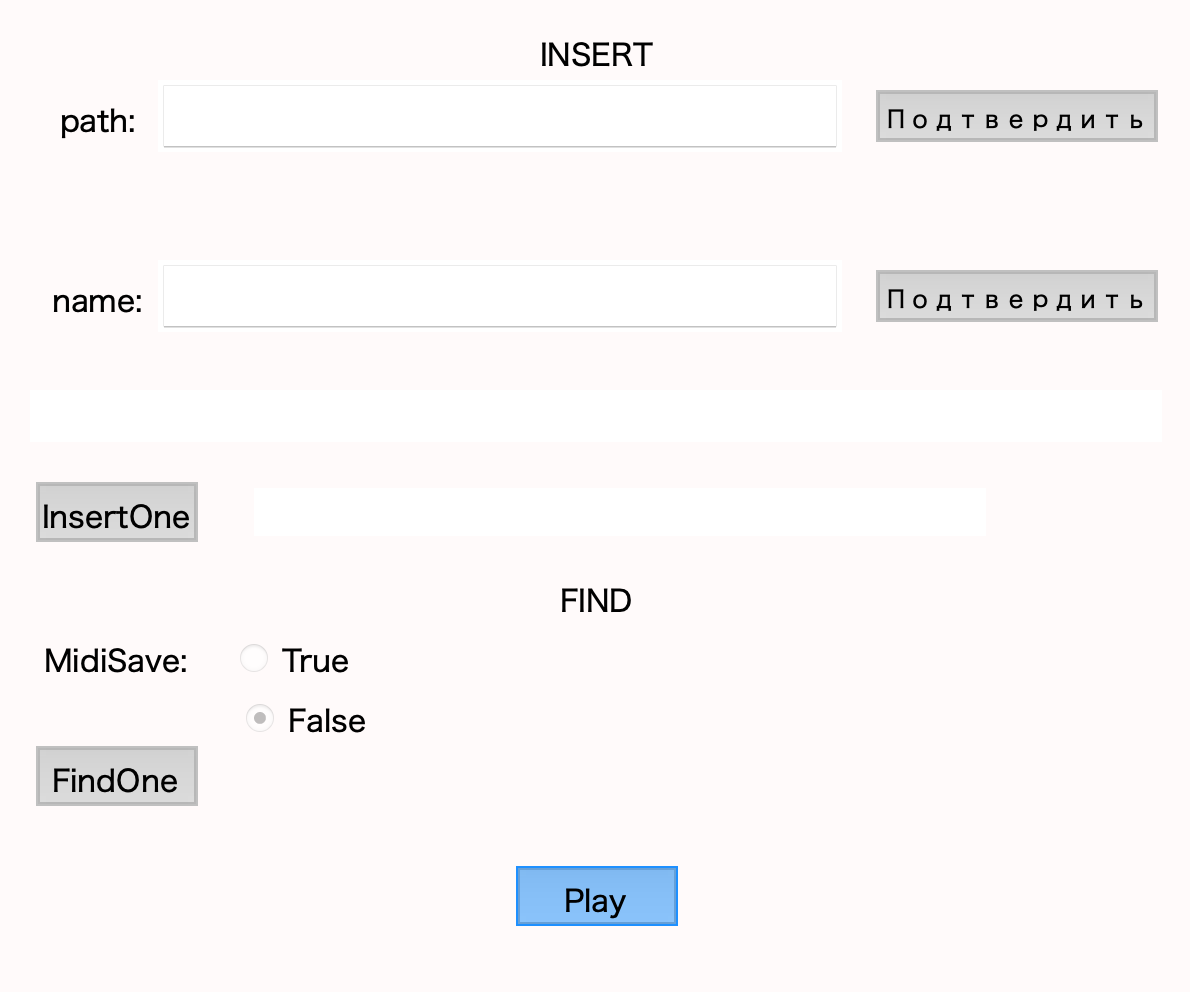
\includegraphics[scale=0.6]{tex/img/Tkinter.png}
		
			Рис 1.3 — Графический интерфейс для демонстрации работы метода
\end{center} 

После заполнения полей path и name будут сформированы данные для запроса к MongoDB на вставку, который бдует выполнен при нажатии на кнопку InsertOne. Результатом успешной операции является идентификатор добавленного в базу данных документа (рис. 1.4). 

\begin{center}
		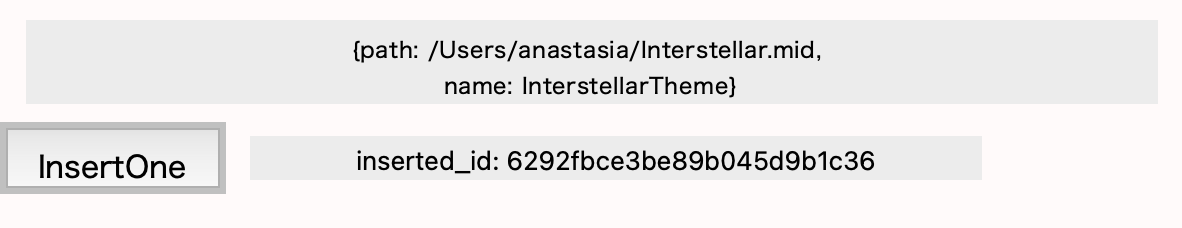
\includegraphics[scale=0.6]{tex/img/Tkinter1.png}
		
			Рис 1.4 — Результат успешного добавления MIDI-файла в MongoDB
\end{center} 

Для извлечения документа с сохранением MIDI-файла полю MidiSave устанавливается значение True. В таком случае документ, извлеченный из базы данных, будет сохранен локально, как файл MIDI с именем InterstellarTheme, который может быть воспроизведен с помощью кнопки Play.

Для удобного просмотра документа в базе данных можно также использовать команду mongosh (листинг \ref{lst:find_command}), где midiFiles -- это коллекция документов.

\begin{lstlisting}[language=sql, label=some-code, caption=Команда mongosh для просмотра документов в MongoDB, label=lst:find_command]
db.midiFiles.find()
\end{lstlisting}

Результатом выполнения этой команды будет вывод всех документов коллекции (в данном случае, одного только что добавленного документа, так как коллекция была пуста) в консоль (рис. 1.5 -- 1.6).

\begin{center}
		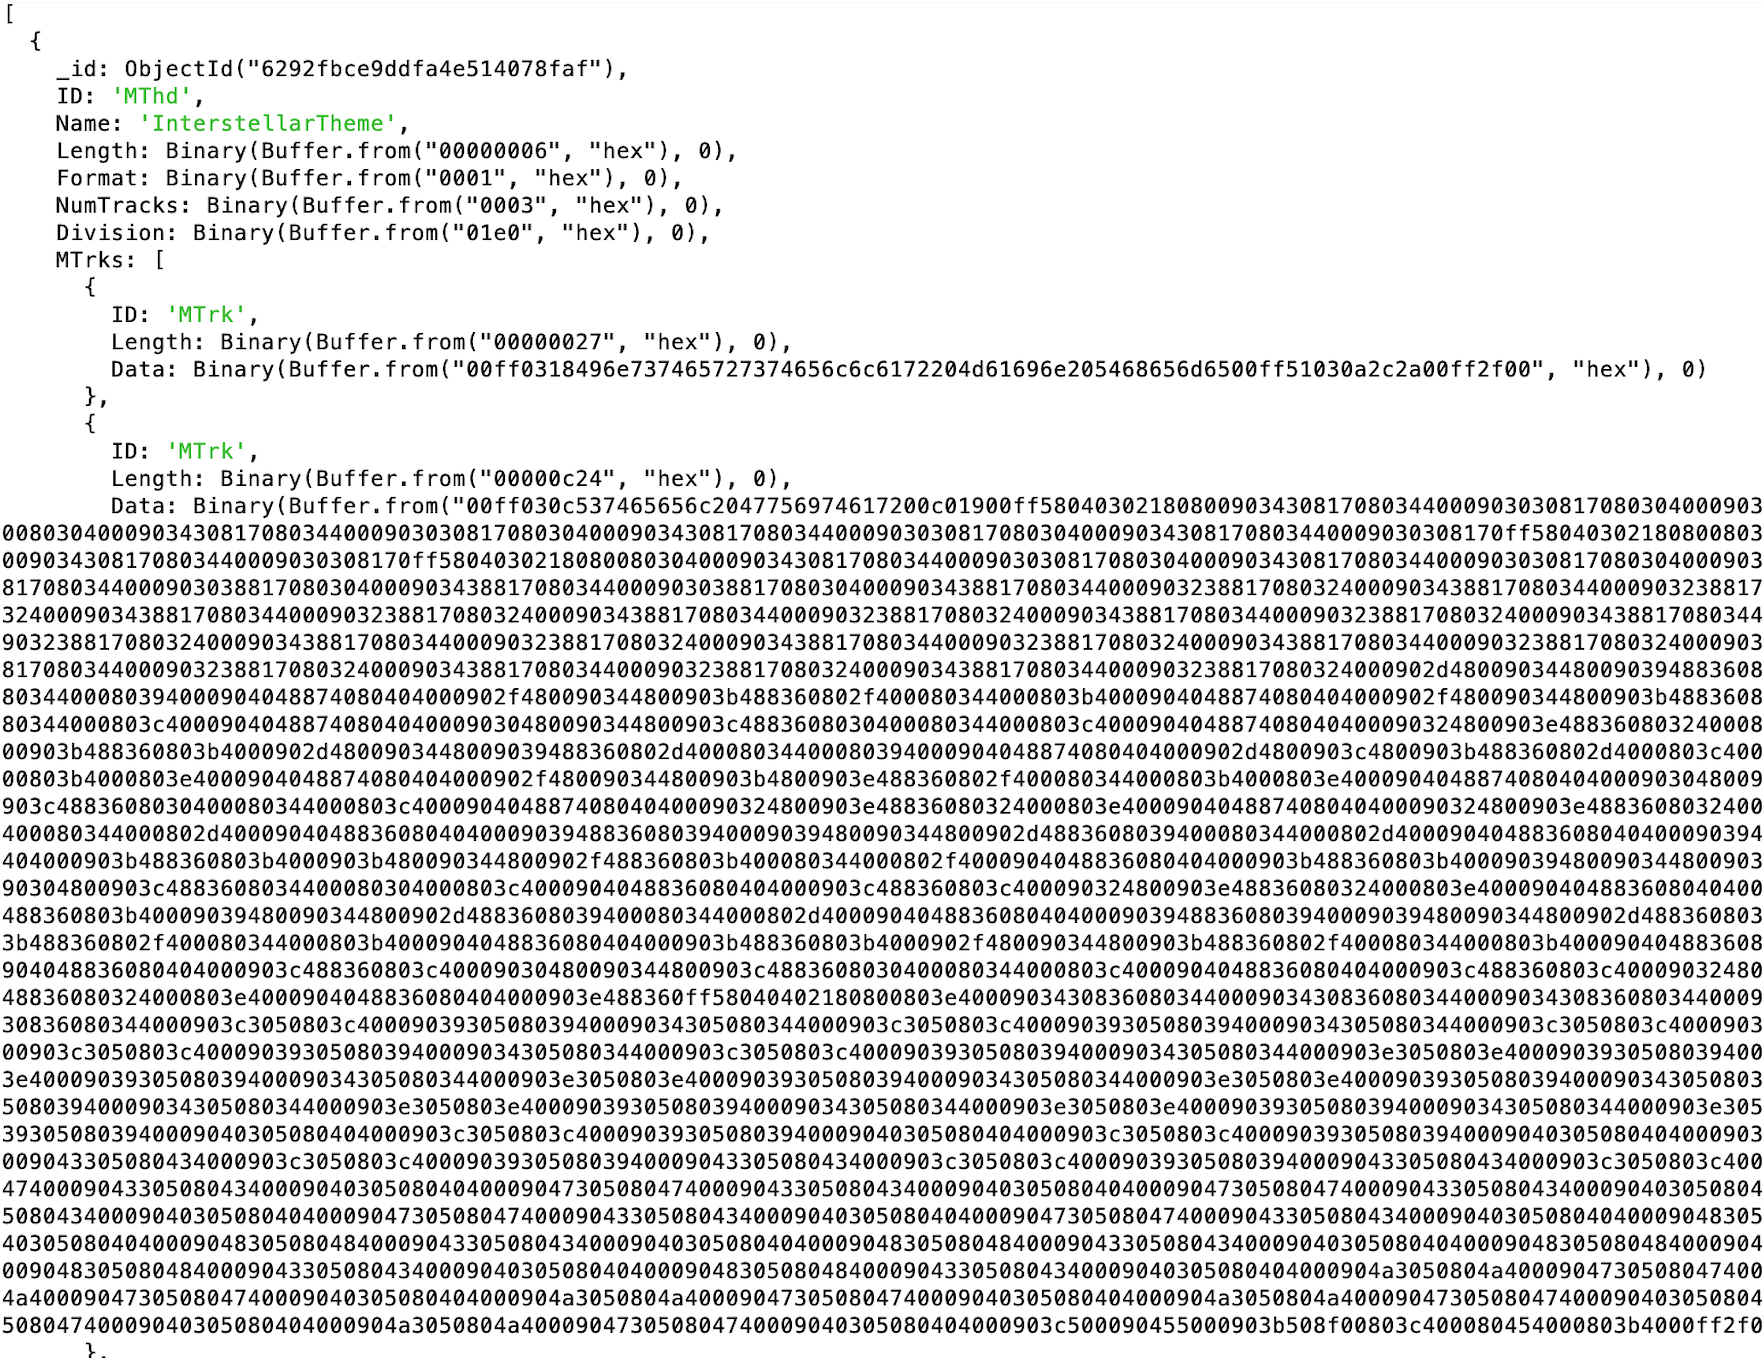
\includegraphics[scale=0.5]{tex/img/Console1.png}
		
			Рис 1.5 — Результат извлечения MIDI-файла из MongoDB (часть 1)
\end{center} 

\begin{center}
		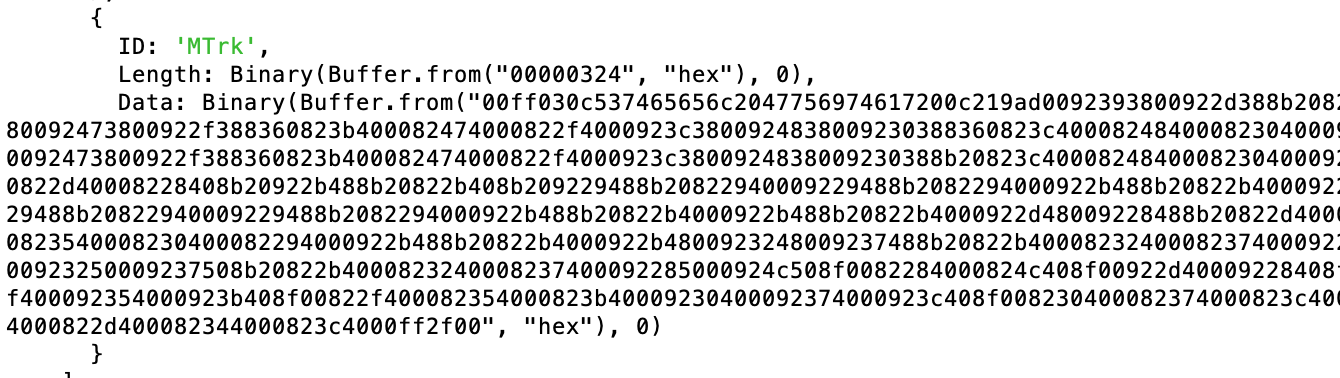
\includegraphics[scale=0.6]{tex/img/Console2.png}
		
			Рис 1.6 — Результат извлечения MIDI-файла из MongoDB (часть 2)
\end{center}


\section{Выводы из технологического раздела}

В данном разделе был обоснован выбор средств программной разработки метода хранения аудио-файлов в NoSQL-базе данных и вспомогательных инструментов для замера времени работы метода и демонстрации его работы. Также была приведена инструкция сборки проекта MongoDB с интегрированным методом и были описаны изменения его структуры. Было проведено тестирование метода с использованием графического интерфейса и интерфейса командной строки.

%%% Local Variables:
%%% mode: latex
%%% TeX-master: "rpz"
%%% End:

\chapter{Исследовательский раздел}

\section{Предмет исследования}

Для проведения исследования работы реализованного метода хранения аудио-файлов в NoSQL-базе данных было составлено 9 MIDI-файлов, отличающихся только количеством музыкальных дорожек (MTrk). Таким образом, первый файл содержит одну музыкальную дорожку, второй - 2, ..., девятый - 9. Данные дорожек не отличаются, в зависимости от их количества незначительно меняется заголовок MIDI-файла: поля Format и NumTracks.
Так, например, аудио-файл, содержащий одну музыкальную дорожку, имеет в базе данных заголовок, представленный на рисунке 4.1.

\begin{center}
		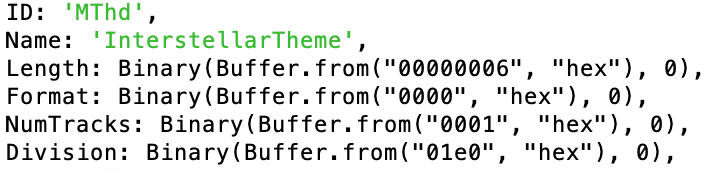
\includegraphics[scale=0.6]{tex/img/OneTrack.png}
		
			Рис 4.1 — Заголовок MIDI-файла, содержащего одну MTrk
\end{center}

Заголвок MIDI-файла с девятью дорожками представлен на рисунке 4.2.
\begin{center}
		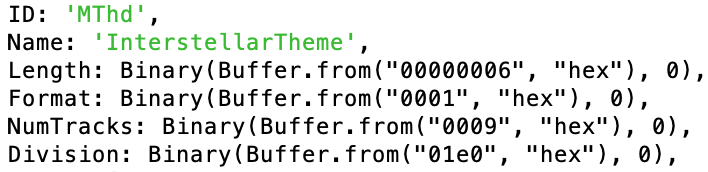
\includegraphics[scale=0.6]{tex/img/NineTracks.png}
		
			Рис 4.2 — Заголовок MIDI-файла, содержащего девять MTrk
\end{center}

Цель исследования - сравнить временные показатели работы с MIDI-файлом при реализованном методе хранения в MongoDB и при хранении его в базе данных в виде неструктурированного массива байтов. Исследуется работа методов хранения при следующих командах базы данных.
\begin{enumerate}
\item Только добавление документа в MongoDB.
\item Только извлечение документа из MongoDB (с последующим доступом к данным самой последней музыкальной дорожки).
\item Добавление и извлечение документа из MongoDB (с последующим доступом к данным самой последней музыкальной дорожки).
\end{enumerate}

В случае реализованного метода распределенного хранения MIDI-файлов, все девять файлов будут храниться в базе данных в виде специальной структуры. Сопоставляемый с ним метод предполагает хранение в виде документа, содержащего один элемент с полем Data, имеющим значение, равное массиву байтов, считанному из аудио-файла. На рисунке 4.3 приведен пример того, как в MongoDB будет представлен такой файл.

\begin{center}
		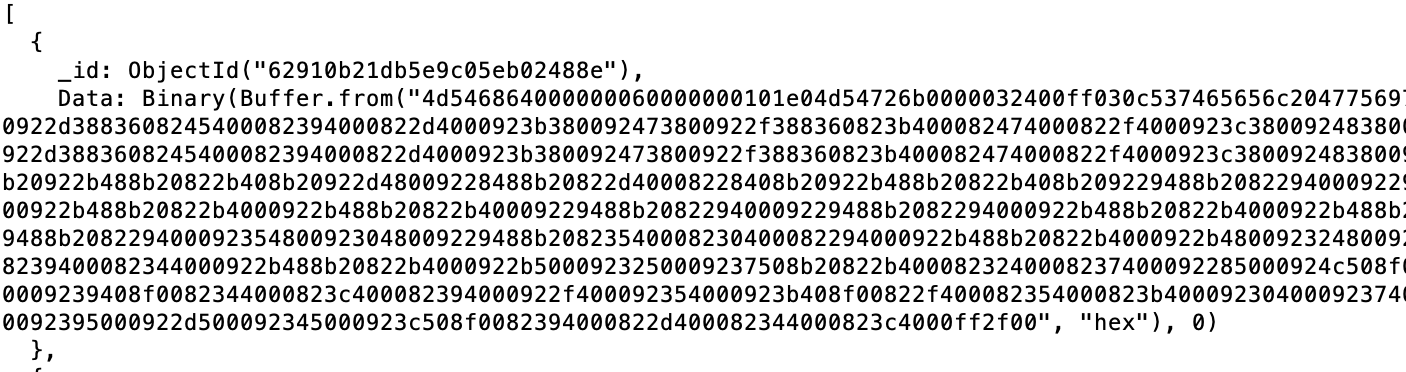
\includegraphics[scale=0.5]{tex/img/Bytes.png}
		
			Рис 4.3 — Метод хранения MIDI-файла в MongoDB в виде массива байтов
\end{center}

\section{Характеристики ЭВМ}

Для исследования использовалась ЭВМ со следующими характеристиками.
\begin{itemize}
	\item MacBook Pro (Retina, 15-inch, Mid 2014).
	\item 2,5 GHz Intel Core i7.
	\item Число логических ядер: 8.
\end{itemize}

\section{Результаты исследования}

\subsection{Добавление документа в MongoDB}

Для добавления MIDI-файла в базу данных для хранения в структурированном виде был реализован метод, формирующий документ MongoDB с помощью пути к аудио-файлу и его имени (листинг \ref{lst:insert_command_test1}). После инициализации документа созданный объект добавляется в базу данных.

\newpage

\begin{lstlisting}[language=C, label=some-code, caption=Добавление MIDI-файла в MongoDB c использованием реализованного метода, label=lst:insert_command_test1]
private async void AddDocument(string number, string name)
        {
            var document = new BsonDocument { { "path", "/Users/anastasia/Desktop/Audiofiles/Interstellar" + number + ".mid" }, 
                { "name", name } };
            _midiCollection.InsertOne(document);
        }
\end{lstlisting}

При вставке массива байтов аудио-файла он считывается из соответствующего файла в переменную array, которая используется для инициализации данных специального типа (бинарный массив) и формирования из них документа MongoDB. По завершении этих действий документ добавляется в базу данных (листинг \ref{lst:insert_command_test2}).

\begin{lstlisting}[language=C, label=some-code, caption=Добавление MIDI-файла в MongoDB в виде массива байтов, label=lst:insert_command_test2]
private async void AddBytesMongoDb(byte[] array)
        {
            var bsonBinaryData = new BsonBinaryData(array);
            var document = new BsonDocument(new BsonElement("Data", bsonBinaryData));
            _midiCollection.InsertOne(document);
        }
\end{lstlisting}

На рисунке 4.4 представлен результат работы методов хранения. Пояснения исследуемых характеристик приведены на рисунке 4.5.

\begin{center}
		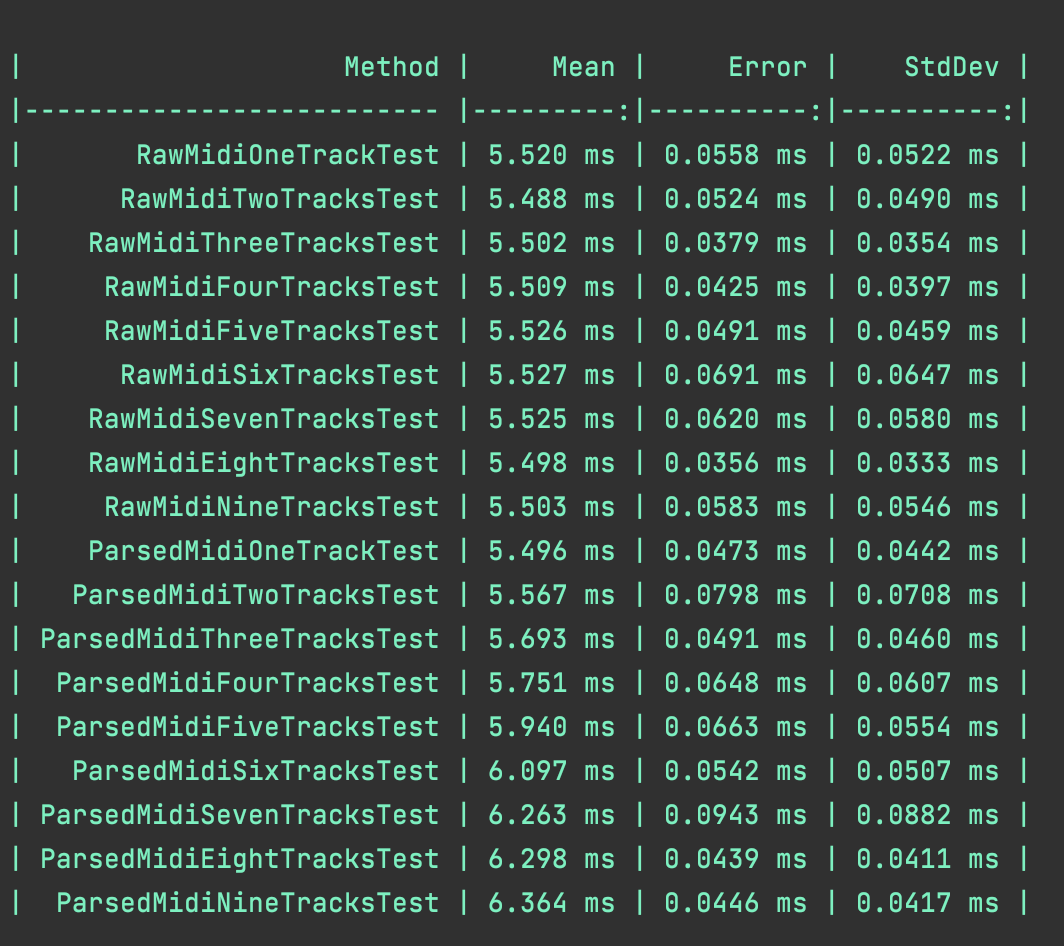
\includegraphics[scale=0.6]{tex/img/InsertClean.png}
		
			Рис 4.4 — Сводная таблица работы методов при добавлении в MongoDB
\end{center}

\begin{center}
		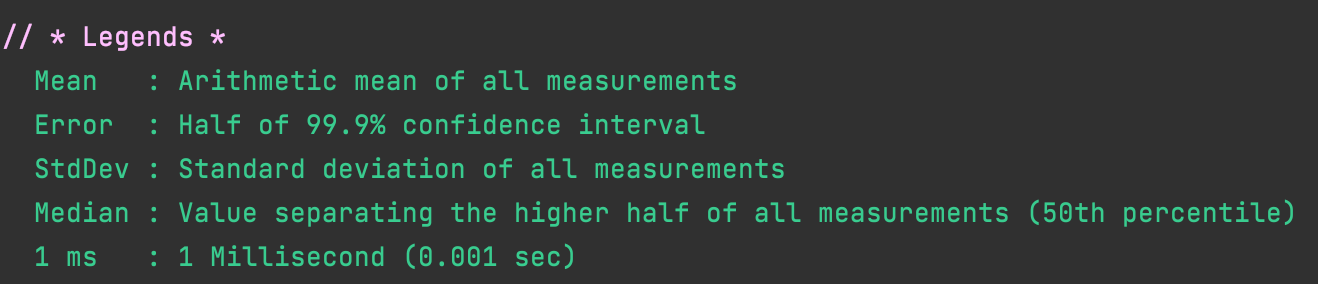
\includegraphics[scale=0.6]{tex/img/Legends.png}
		
			Рис 4.5 — Сводная таблица работы методов при добавлении в MongoDB
\end{center}

На рисунке 4.6 полученные временные характеристики представлены в графическом виде.

\begin{center}
		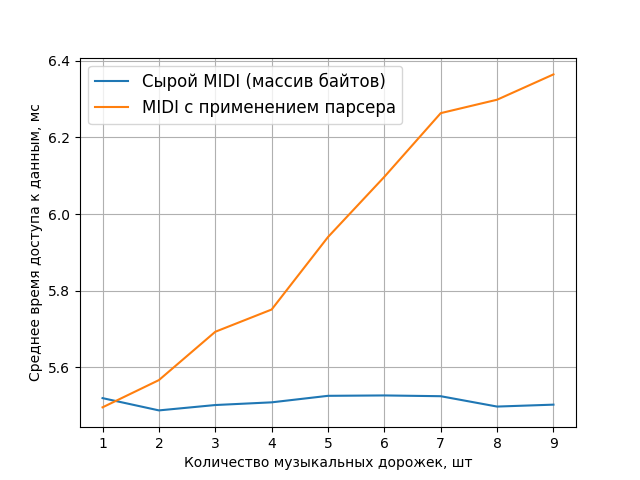
\includegraphics[scale=0.7]{tex/img/figure_insert_query.png}
		
			Рис 4.6 — Сравнение работы методов при добавлении в MongoDB
\end{center}

Как видно из рисунков 4.4 и 4.6, наибольшая скорость работы операции добавления документа в MongoDB достигается при использовании метода хранения MIDI-файла на основе его содержания. Однако, при увеличении количества музыкальных дорожек время работы этого метода растет пропорционально числу дорожек, что объясняется тем, что каждый раз при вставке аудио-файла в базу данных применяется парсер. Скорость роста составляет примерно 0,096 мс/шт. Таким образом, реализация хранения в виде массива байтов имеет выигрыш по временной эффективности приблизительно в 1,2 раза.

\subsection{Извлечение документа из MongoDB}

Для извлечения MIDI-файла из базы данных и доступа к его последней дорожке, в случае хранения в структурированном виде, требуется только обращение к документу MongoDB с поиском значения нужного поля (листинг \ref{lst:find_command_test1}). 

\newpage

\begin{lstlisting}[language=C, label=some-code, caption=Извлечение MIDI-файла из MongoDB c использованием реализованного метода, label=lst:find_command_test1]
var documents = _midiCollection.Find(new BsonDocument()).ToList();
var parsedDocument = documents.Last();

var result =  parsedDocument.GetElement("MTrks").Value.AsBsonArray.Last().AsBsonDocument
    .GetElement("Data").Value.AsByteArray;
\end{lstlisting}

При извлечении массива байтов аудио-файла, чтобы найти нужные данные, сначала нужно применить парсер, который преобразует бинарный объект в определенную структуру, по которой можно выполнить поиск. Метод ParseMidiFile использует ту же структуру и средства, что и парсер, используемый в разработанном методе хранения (листинг \ref{lst:find_command_test2}).

\begin{lstlisting}[language=C, label=some-code, caption=Извлечение MIDI-файла из MongoDB в виде массива байтов, label=lst:find_command_test2]
var documents = _midiCollection.Find(new BsonDocument()).ToList();
var rawDocument = documents.Last();

var midiFileRaw = rawDocument.GetElement("Data").Value.AsByteArray;
var midiFile = _midiFileParser.ParseMidiFile(midiFileRaw);
var result = midiFile.MTrks.Last().Data;
\end{lstlisting}

На рисунке 4.7 представлен результат работы методов хранения. Пояснения исследуемых характеристик приведены на рисунке 4.5.

\begin{center}
		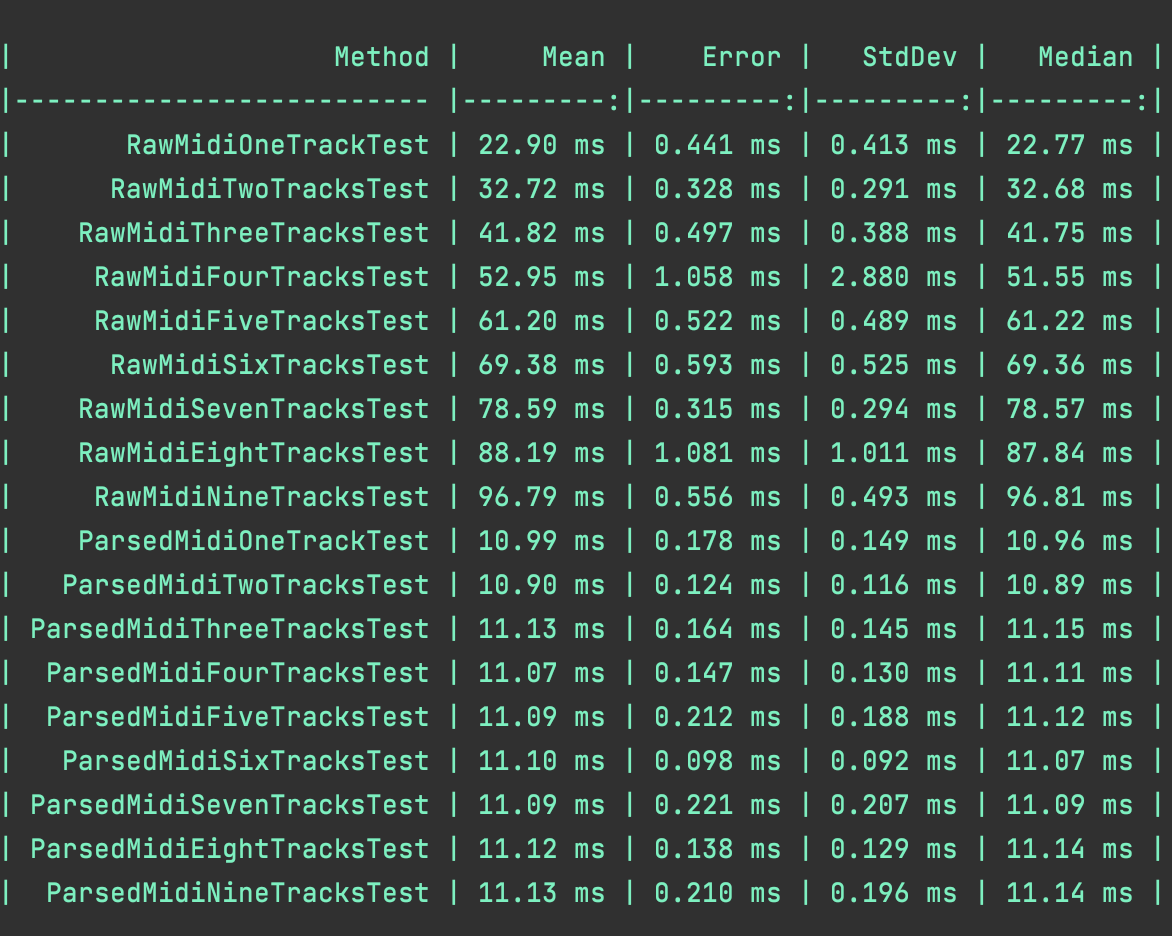
\includegraphics[scale=0.6]{tex/img/FindClean.png}
		
			Рис 4.7 — Сводная таблица работы методов при извлечении из MongoDB
\end{center}

На рисунке 4.8 полученные временные характеристики представлены в графическом виде.

\begin{center}
		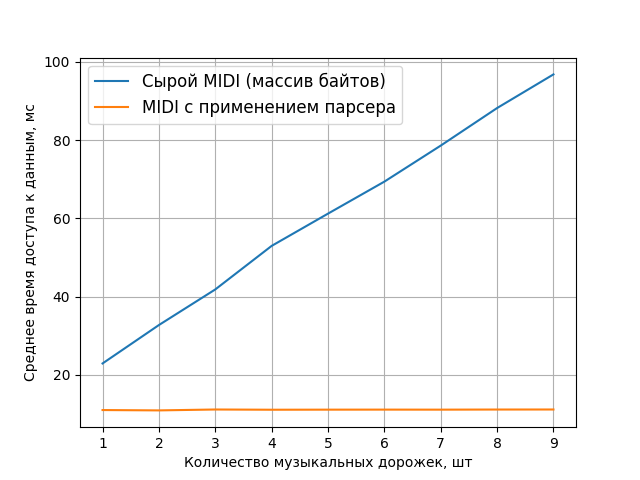
\includegraphics[scale=0.7]{tex/img/figure_find_query.png}
		
			Рис 4.8 — Сравнение работы методов при извлечении из MongoDB
\end{center}

Из рисунков 4.7 и 4.8 видно, что наибольшая скорость выполнения операции чтения документа из MongoDB достигается при использовании метода хранения MIDI-файла в структурированном виде. При этом скорость работы почти не меняется при увеличении числа музыкальных дорожек, разница во времени выполнения доступа к данным при девяти дорожках и одной дорожке составляет 0,14 миллисекунд. Время работы доступа к данным при методе хранения массива байтов, наоборот, растет из-за накладных расходов применяемого парсера. Скорость роста составляет 8,21 мс/шт. Таким образом, реализация хранения в виде структуры MIDI-файла имеет выигрыш по временной эффективности приблизительно в 8,7 раза.

\subsection{Добавление и извлечение документа из MongoDB}

Для оценки времени работы обеих операций добавления и извлечения документов из MongoDB при разных подходах к хранению данных использовались описанные выше методы в совокупности. 
Для исследования добавления и извлечения MIDI-файла, хранящегося в виде струкутры, были использованы методы, представленные на листинге \ref{lst:insert_find_command_test1}. 

\begin{lstlisting}[language=C, label=some-code, caption=Добавление и извлечение MIDI-файла из MongoDB c использованием реализованного метода, label=lst:insert_find_command_test1]
AddDocument("1", "Interstellar1");

var documents = _midiCollection.Find(new BsonDocument()).ToList();
var parsedDocument = documents.Last();

var result =  parsedDocument.GetElement("MTrks").Value.AsBsonArray.Last().AsBsonDocument
    .GetElement("Data").Value.AsByteArray;
\end{lstlisting}

Для исследования добавления и извлечения MIDI-файла, хранящегося в виде массива байтов, были использованы методы, представленные на листинге \ref{lst:insert_find_command_test2}.

\newpage

\begin{lstlisting}[language=C, label=some-code, caption=Добавление и извлечение MIDI-файла из MongoDB в виде массива байтов, label=lst:insert_find_command_test2]

AddBytesMongoDb(FileOperations
    .ReadFileAsync("/Users/anastasia/Interstellar1.mid"));

var documents = _midiCollection.Find(new BsonDocument()).ToList();
var rawDocument = documents.Last();

var midiFileRaw = rawDocument.GetElement("Data").Value.AsByteArray;
var midiFile = _midiFileParser.ParseMidiFile(midiFileRaw);
var result = midiFile.MTrks.Last().Data;
\end{lstlisting}

На рисунке 4.9 представлен результат работы методов хранения. Пояснения исследуемых характеристик приведены на рисунке 4.5.

\begin{center}
		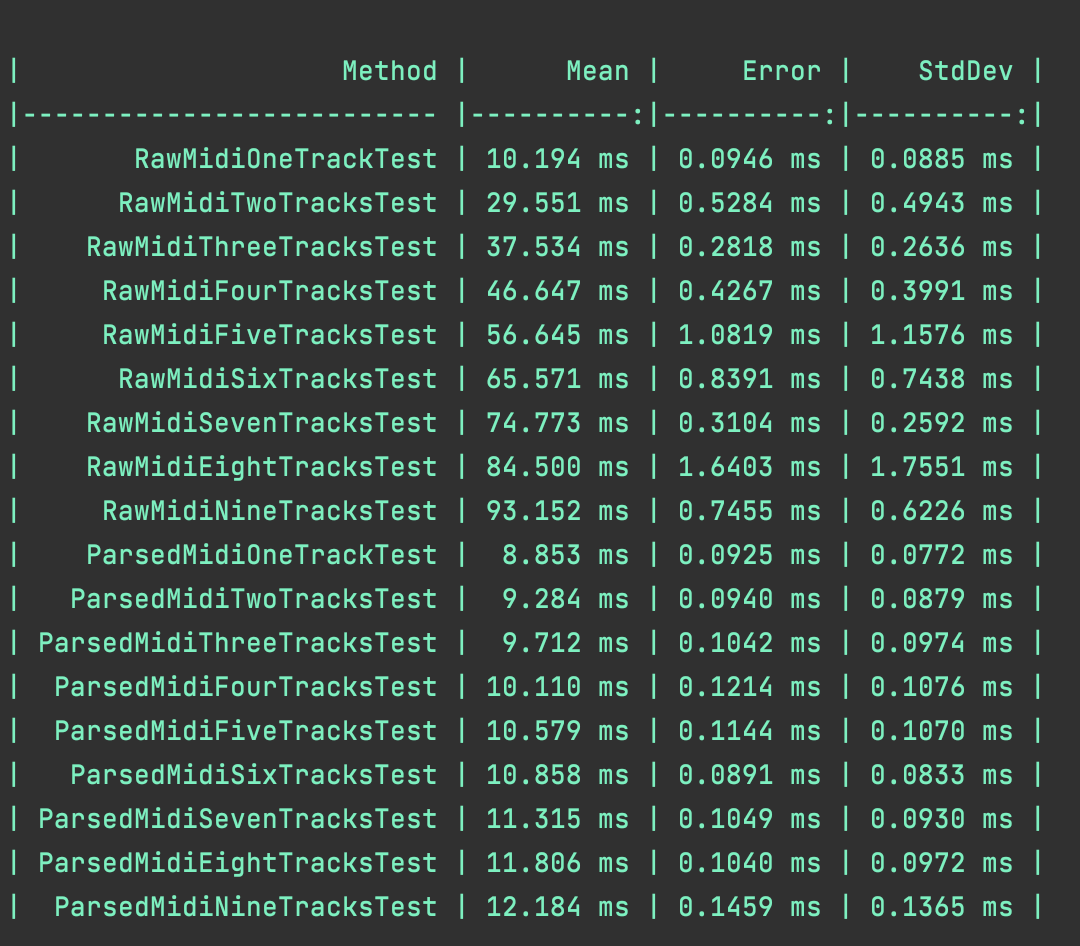
\includegraphics[scale=0.6]{tex/img/InsertFindClean.png}
		
			Рис 4.9 — Сводная таблица работы методов при извлечении из MongoDB
\end{center}

На рисунке 4.10 полученные временные характеристики представлены в графическом виде.

\begin{center}
		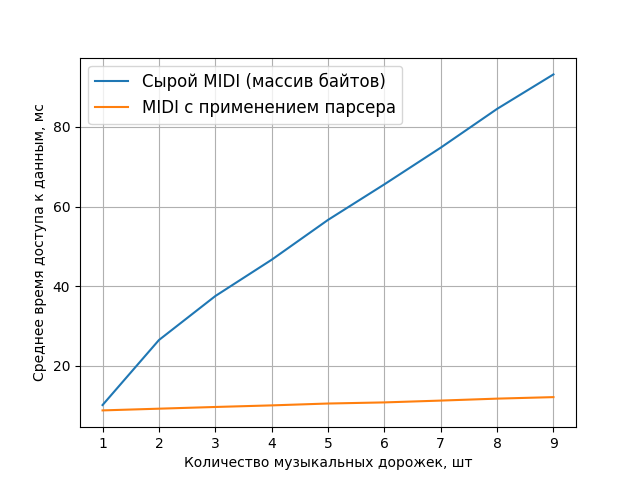
\includegraphics[scale=0.7]{tex/img/figure_find_insert_query.png}
		
			Рис 4.10 — Сравнение работы методов при добавлении и извлечении из MongoDB
\end{center}

Из рисунков 4.9 и 4.10 очевидно, что наибольшая скорость работы операций записи и чтения документа из MongoDB достигается при использовании метода хранения MIDI-файла в структурированном виде. Время работы метода медленно растет при увеличении числа музыкальных дорожек, а скорость роста составляет приблизительно 0,37 мс/шт. Время работы операций записи и чтения при методе хранения массива байтов резко растет, и скорость роста составляет примерно 9,22 мс/шт. Таким образом, реализация хранения MIDI-файла в виде его структуры имеет выигрыш по временной эффективности приблизительно в 7,6 раза. 

\section{Выводы из исследовательского раздела}

В данном разделе было проведено исследование временных характеристик работы операций добавления и извлечения документа из MongoDB при двух способах хранения: с использованием разработанного метода и без использования разработанного метода (хранение в виде массива байтов). По результатам исследования, метод распределенного хранения MIDI-файла в виде его структуры показал немного меньшую эффективность при операции добавления в MongoDB, но значительно большую эффективность при операции извлечения данных, а также при работе обеих этих операций в совокупности. 

%%% Local Variables:
%%% mode: latex
%%% TeX-master: "rpz"
%%% End:

% \chapter{Организационно-экономический раздел}
\label{cha:econom}

\section{Протестируем специальные символы.}

И заодно переключение шрифтов.


{\shorthandoff" \texttt{"-{}-* Прямая речь "-{}-{}- <{}<после ,{},тире`{}` неразрывный пробел>{}>}}

{\cyrillicfonttt{\bfseries\itshape\textbackslash{}cyrillicfonttt}
"--* Прямая речь "--- <<после ,,тире`` неразрывный пробел>>.}

{\cyrillicfontsf{\bfseries\itshape\textbackslash{}cyrillicfontsf}
"--* Прямая речь "--- <<после ,,тире`` неразрывный пробел>>.}

{\cyrillicfont{\bfseries\itshape\textbackslash{}cyrillicfont}
"--* Прямая речь "--- <<после ,,тире`` неразрывный пробел>>.}


\blindtext
%%% Local Variables:
%%% mode: latex
%%% TeX-master: "rpz"
%%% End:

% \chapter{Промышленная экология и безопасность}\label{cha:bzd}

\blindtext

\blindlistlist[3]{enumerate}

%%% Local Variables:
%%% mode: latex
%%% TeX-master: "rpz"
%%% End:


\backmatter %% Здесь заканчивается нумерованная часть документа и начинаются ссылки и
            
\Conclusion % заключение к отчёту

В ходе работе проанализированы существующие аудио-форматы, выбран аудио-формат, дающий наиболее полную информацию о музыке, проанализированы существующие решения хранения такого формата в различных базах данных и выбран способ хранения, наиболее оптимальный для выбранного формата, проанализированы существующие модели данных и выбрана наиболее подходящая под выбранный способ хранения модель, а также выбрана база данных, которая ее использует. Разработано программное обеспечение, реализующее описанный метод. Произведено исследование времени работы метода и проанализированы полученные результаты.

В рамках работы были решены все поставленные задачи.
\begin{enumerate}
    \item Рассмотрены способы представления звуковой информации и проанализированы существующие аудио-форматы.
    \item Проанализированы способы хранения аудио-файлов в различных базах данных.
    \item Разработан метод хранения аудио-файлов.
    \item Разработано программное обеспечение, реализующее разработанный метод.
    \item Исследована зависимость времени работы метода от количества дорожек в аудио-файле.
\end{enumerate}




%%% Local Variables: 
%%% mode: latex
%%% TeX-master: "rpz"
%%% End: 
%% заключение

%% % Список литературы при помощи BibTeX
% Юзать так:
%
% pdflatex rpz
% bibtex rpz
% pdflatex rpz
\bibliographystyle{gost780u}
\bibliography{rpz}


%%% Local Variables: 
%%% mode: latex
%%% TeX-master: "rpz"
%%% End: 

\bibliographystyle{gost780u}
\bibliography{bibliography.bib}

\chapter{ПРИЛОЖЕНИЕ А}
\parindent = 1.25cm
%Файл классификации:
%\lstinputlisting[firstline=4,lastline=79]{Classification.py}
%Файл нахождение дуги и аппроксимации:
%\lstinputlisting[firstline=171,lastline=289]{Learning.py}

\begin{lstlisting}[language=C, label=some-code, caption=Метод создания  документа MongoDB по спецификации MIDI (часть 1), label=lst:parser_midi1]
BSONObj parseMidiFile(const vector<char> buffer, const string fileName) {
    BSONObjBuilder builder;
    int i;
    int i_buff;

    // MThd ID
    char MThdId[5];
    for (i_buff = 0, i = 0; i_buff < 4; i_buff++, i++) {
        MThdId[i] = buffer[i_buff];
    }
    builder.append("ID", MThdId);

    builder.append("Name", fileName);

    // MThd Length
    char MThdLength[5];
    for (i_buff = 4, i = 0; i_buff < 8; i_buff++, i++) {
        MThdLength[i] = buffer[i_buff];
    }
    builder.appendBinData("Length", 4, BinDataGeneral, MThdLength);

    // MThd Format
    char MThdFormat[3];
    for (i_buff = 8, i = 0; i_buff < 10; i_buff++, i++) {
        MThdFormat[i] = buffer[i_buff];
    }
    builder.appendBinData("Format", 2, BinDataGeneral, MThdFormat);

    // MThd NumTracks
    char MThdNumTracks[3];
    for (i_buff = 10, i = 0; i_buff < 12; i_buff++, i++) {
        MThdNumTracks[i] = buffer[i_buff];
    }
    builder.appendBinData("NumTracks", 2, BinDataGeneral, MThdNumTracks);

    // MThd Division
    char MThdDivision[3];
    for (i_buff = 12, i = 0; i_buff < 14; i_buff++, i++) {
        MThdDivision[i] = buffer[i_buff];
    }
    builder.appendBinData("Division", 2, BinDataGeneral, MThdDivision);
\end{lstlisting}

\begin{lstlisting}[language=C, label=some-code, caption=Метод создания  документа MongoDB по спецификации MIDI (часть 2), label=lst:parser_midi2] 
    // MThd MTrks
    const int numTracks = convertByteToIntMthd(MThdNumTracks);
    BSONArray mtrks = BSONArray();
    int mtrkBegin = i_buff;
    int mtrkOffset = i_buff;
    int j;
    int i_mtrk;

    BSONObjBuilder mtrksBuilder(builder.subarrayStart("MTrks"));
    for (i_mtrk = 0; i_mtrk < numTracks; i_mtrk++) {
        BSONObjBuilder mtrkBuilder(mtrksBuilder.subobjStart("mtrk"));
        // MTrk ID
        char MTrkId[5];
        mtrkOffset += 4;
        for (j = mtrkBegin, i = 0; j < mtrkOffset; j++, i++) {
            MTrkId[i] = buffer[j];
        }
        mtrkBuilder.append("ID", MTrkId);

        mtrkBegin = mtrkOffset;
        mtrkOffset += 4;

        // MTrk Length
        char MTrkLength[5];
        for (j = mtrkBegin, i = 0; j < mtrkOffset; j++, i++) {
            MTrkLength[i] = buffer[j];
        }
        mtrkBuilder.appendBinData("Length", 4, BinDataGeneral, MTrkLength);
        const int mtrkLengthInt = convertByteToIntMtrk(MTrkLength);

        mtrkBegin = mtrkOffset;
        mtrkOffset += mtrkLengthInt;

        // MTrk Data
        char* Data = new char[mtrkLengthInt];
        for (j = mtrkBegin, i = 0; j < mtrkOffset; j++, i++) {
            Data[i] = buffer[j];
        }
        mtrkBuilder.appendBinData("Data", mtrkLengthInt, BinDataGeneral, Data);

        mtrkBegin = mtrkOffset;
\end{lstlisting}

\begin{lstlisting}[language=C, label=some-code, caption=Метод создания  документа MongoDB по спецификации MIDI (часть 3), label=lst:parser_midi3] 
        mtrkBuilder.done();
    }
    mtrksBuilder.done();
    BSONObj midi = builder.obj();

    return midi;
}
\end{lstlisting}

%%% Local Variables: 
%%% mode: latex
%%% TeX-master: "rpz"
%%% End: 

\chapter{ПРИЛОЖЕНИЕ Б}
\parindent = 1.25cm
%Файл классификации:
%\lstinputlisting[firstline=4,lastline=79]{Classification.py}
%Файл нахождение дуги и аппроксимации:
%\lstinputlisting[firstline=171,lastline=289]{Learning.py}

\begin{lstlisting}[language=C, label=some-code, caption=Метод записи документа MongoDB в MIDI-файл (часть 1), label=lst:file_builder1]
std::string parseMidiRecord(const BSONObj& doc) {
    BSONObjIterator iter(doc);

    BSONElement elem;
    const char* bytes;
    const char* fieldName;
    const char* fileName;
    std::string buffer;
    int len;

    while (iter.more()) {
        elem = iter.next();
        fieldName = elem.fieldName();
        if (strcmp(fieldName, "_id") == 0)
            continue;
        if (strcmp(fieldName, "Name") == 0) {
            fileName = elem.valueStringDataSafe().rawData();
            continue;
        }

        BSONType t;
        
        t = elem.type();
        if (t == Object || t == Array) {
            BSONObj subObj = elem.embeddedObject();
            BSONElement subElem;
            BSONObjIterator subObjIter(subObj);

            while (subObjIter.more()) {
                subElem = subObjIter.next();

                t = subElem.type();
                if (t == Object || t == Array) {
                    BSONObj mtrks = subElem.embeddedObject();
                    BSONElement mtrk;
                    BSONObjIterator mtrkIter(mtrks);

                    while (mtrkIter.more()) {
                        mtrk = mtrkIter.next();
                        t = mtrk.type();
                        bytes = getBsonElementValue(t, mtrk);
                        len = mtrk.valuesize() - 5;
\end{lstlisting}

\begin{lstlisting}[language=C, label=some-code, caption=Метод записи документа MongoDB в MIDI-файл (часть 2), label=lst:file_builder2]
                        for (int i = 0; i < len; i++) {
                            buffer += bytes[i];
                        }
                    }
                }
            }
        } else {
            len = elem.valuesize() - 5;
            bytes = getBsonElementValue(t, elem);

            for (int i = 0; i < len; i++) {
                buffer += bytes[i];
            }
        }
    }
    return buffer;
}
\end{lstlisting}

%%% Local Variables: 
%%% mode: latex
%%% TeX-master: "rpz"
%%% End: 

\end{document}

%%% Local Variables:
%%% mode: latex
%%% TeX-master: t
%%% End:
